% ==================== %
% == RESOURCES USED == %
% ==================== %


\begin{filecontents*}[overwrite]{gallery-showcase-bw.tex}
\documentclass[theme = bw]{tutodoc}

% == FORDOC == %

\usepackage{multicol}
\usepackage{lastpage}

\renewcommand*\pagemark{%
  \usekomafont{pagenumber}{\thepage\kern1pt/\kern1pt\pageref*{LastPage}}%
}


\newcommand\thisstyle{bw}


\newcommand\myexrmktext{
    \tdocversion{1.7.0}[2024-12-04]
    In the flow of the text, it is always useful to be able to provide examples and comments to supplement the main content.
}


\newcommand\myadmotext{
    Depending on the context of use, it is sometimes necessary to be able to highlight content by indicating its degree of importance.
}

\newcommand\myhighlightedtextnonote{
    What to say?
    I don't know, but it's nice. No ?
}

\newcommand\myhighlightedtext{
    What to say
    \footnote{
        Let's not forget the footnotes...
    }?
    I don't know, but it's nice. No ?
}


\newcommand\mychgestext{
    In a change log, it is important to visualise the types of changes clearly. This makes it easier for the user to read!
}


\ExplSyntaxOn

\int_new:N \g__tutodoc_for_doc_int

\ExplSyntaxOff



\begin{document}

\textsf{\Huge\bfseries The \texttt{"\thisstyle"} theme}

\section{Liens}

{\Large\bfseries \href{https://github.com/bc-tools/for-latex/tree/main/tutodoc}{A very big link}}, but at least we can see it.



\section{\LaTeX\ listings}

Typing in on-line code such as \tdoclatexin{E = m c^2 \neq \pi \neq \frac{3}{14}} is useful, as is showing use cases such as the following one.

\begin{tdoclatex}
Formatted \LaTeX\ code is great: $E = m c^2$ or $pi \neq \frac{3}{14}$.
\end{tdoclatex}


There's also a less invasive side-by-side mode. Nice! No ?

\begin{tdoclatex}[\tdoctcb{sbs}]
Formatted \LaTeX\ code is great:       \\
$E = m c^2$ or $\pi \neq \frac{3}{14}$.
\end{tdoclatex}



\section{Highlighting, versioning and dating}

\subsection{tdocexa, tdocrem}

\myexrmktext

\ExplSyntaxOn

\seq_map_inline:Nn \g__tutodoc_focus_std_seq {
    \begin{tdoc#1}
        \myhighlightedtext
    \end{tdoc#1}
}

\ExplSyntaxOff



\subsection{tdocnote, tdoctip...}

\myadmotext

\ExplSyntaxOn

\int_set:Nn \g__tutodoc_for_doc_int { 0 }

\ifcsundef{g__tutodoc_focus_color_seq}{
    \prop_map_inline:Nn \g__tutodoc_focus_color_prop {
        \int_gincr:N \g__tutodoc_for_doc_int

        \begin{tdoc#1}
      	  	\int_compare:nTF
	    		{\g__tutodoc_for_doc_int = 1 }
	    		{ \myhighlightedtext }
	    		{ \myhighlightedtextnonote }
        \end{tdoc#1}
    }
} {
    \seq_map_inline:Nn \g__tutodoc_focus_color_seq {
        \int_gincr:N \g__tutodoc_for_doc_int

        \begin{tdoc#1}
      	  	\int_compare:nTF
	    		{\g__tutodoc_for_doc_int = 1 }
	    		{ \myhighlightedtext }
	    		{ \myhighlightedtextnonote }
        \end{tdoc#1}
    }
}

\ExplSyntaxOff



\subsection{tdocbreak, tdocfix...}

\tdocstartproj{A new demonstration section...}

\begin{tdoctodo}
	\item A gallery would be welcome...
\end{tdoctodo}

\ifcsundef{g__tutodoc_topic_change_seq}{
 	\medskip
}{}

\mychgestext

\ifcsundef{g__tutodoc_topic_change_seq}{
	\medskip
}{}

\ExplSyntaxOn

\int_set:Nn \g__tutodoc_for_doc_int { 0 }

\begin{tabular}{%
	@{\hskip 0pt}p{.26\linewidth}%
	*{3}{@{\hskip 7pt}p{.23\linewidth}}@{\hskip 0pt}%
}
	\ifcsundef{g__tutodoc_topic_change_seq}{
    	\prop_map_inline:Nn \g__tutodoc_topic_change_prop {
          	\int_gincr:N \g__tutodoc_for_doc_int

          	\vspace{-12pt}

    	  	\begin{tdoc#1}
           		\item Infos...
    	  	\end{tdoc#1}

    	  	\int_compare:nTF
    	    	{\g__tutodoc_for_doc_int = 4 }
    	    	{ \\ }
    	    	{ & }
    	}
	}{
    	\seq_map_inline:Nn \g__tutodoc_topic_change_seq {
          	\int_gincr:N \g__tutodoc_for_doc_int

          	\vspace{-5pt}

    	  	\begin{tdoc#1}
           		\item Infos...
    	  	\end{tdoc#1}

    	  	\int_compare:nTF
    	    	{\g__tutodoc_for_doc_int = 4 }
    	    	{ \\ }
    	    	{ & }
    	}
	}
\end{tabular}

\ExplSyntaxOff

\end{document}

\end{filecontents*}

\begin{filecontents*}[overwrite]{gallery-showcase-color.tex}
\documentclass[theme = color]{tutodoc}

% == FORDOC == %

\usepackage{multicol}
\usepackage{lastpage}

\renewcommand*\pagemark{%
  \usekomafont{pagenumber}{\thepage\kern1pt/\kern1pt\pageref*{LastPage}}%
}


\newcommand\thisstyle{color}


\newcommand\myexrmktext{
    \tdocversion{1.7.0}[2024-12-04]
    In the flow of the text, it is always useful to be able to provide examples and comments to supplement the main content.
}


\newcommand\myadmotext{
    Depending on the context of use, it is sometimes necessary to be able to highlight content by indicating its degree of importance.
}

\newcommand\myhighlightedtextnonote{
    What to say?
    I don't know, but it's nice. No ?
}

\newcommand\myhighlightedtext{
    What to say
    \footnote{
        Let's not forget the footnotes...
    }?
    I don't know, but it's nice. No ?
}


\newcommand\mychgestext{
    In a change log, it is important to visualise the types of changes clearly. This makes it easier for the user to read!
}


\ExplSyntaxOn

\int_new:N \g__tutodoc_for_doc_int

\ExplSyntaxOff



\begin{document}

\textsf{\Huge\bfseries The \texttt{"\thisstyle"} theme}

\section{Liens}

{\Large\bfseries \href{https://github.com/bc-tools/for-latex/tree/main/tutodoc}{A very big link}}, but at least we can see it.



\section{\LaTeX\ listings}

Typing in on-line code such as \tdoclatexin{E = m c^2 \neq \pi \neq \frac{3}{14}} is useful, as is showing use cases such as the following one.

\begin{tdoclatex}
Formatted \LaTeX\ code is great: $E = m c^2$ or $pi \neq \frac{3}{14}$.
\end{tdoclatex}


There's also a less invasive side-by-side mode. Nice! No ?

\begin{tdoclatex}[\tdoctcb{sbs}]
Formatted \LaTeX\ code is great:       \\
$E = m c^2$ or $\pi \neq \frac{3}{14}$.
\end{tdoclatex}



\section{Highlighting, versioning and dating}

\subsection{tdocexa, tdocrem}

\myexrmktext

\ExplSyntaxOn

\seq_map_inline:Nn \g__tutodoc_focus_std_seq {
    \begin{tdoc#1}
        \myhighlightedtext
    \end{tdoc#1}
}

\ExplSyntaxOff



\subsection{tdocnote, tdoctip...}

\myadmotext

\ExplSyntaxOn

\int_set:Nn \g__tutodoc_for_doc_int { 0 }

\ifcsundef{g__tutodoc_focus_color_seq}{
    \prop_map_inline:Nn \g__tutodoc_focus_color_prop {
        \int_gincr:N \g__tutodoc_for_doc_int

        \begin{tdoc#1}
      	  	\int_compare:nTF
	    		{\g__tutodoc_for_doc_int = 1 }
	    		{ \myhighlightedtext }
	    		{ \myhighlightedtextnonote }
        \end{tdoc#1}
    }
} {
    \seq_map_inline:Nn \g__tutodoc_focus_color_seq {
        \int_gincr:N \g__tutodoc_for_doc_int

        \begin{tdoc#1}
      	  	\int_compare:nTF
	    		{\g__tutodoc_for_doc_int = 1 }
	    		{ \myhighlightedtext }
	    		{ \myhighlightedtextnonote }
        \end{tdoc#1}
    }
}

\ExplSyntaxOff



\subsection{tdocbreak, tdocfix...}

\tdocstartproj{A new demonstration section...}

\begin{tdoctodo}
	\item A gallery would be welcome...
\end{tdoctodo}

\ifcsundef{g__tutodoc_topic_change_seq}{
 	\medskip
}{}

\mychgestext

\ifcsundef{g__tutodoc_topic_change_seq}{
	\medskip
}{}

\ExplSyntaxOn

\int_set:Nn \g__tutodoc_for_doc_int { 0 }

\begin{tabular}{%
	@{\hskip 0pt}p{.26\linewidth}%
	*{3}{@{\hskip 7pt}p{.23\linewidth}}@{\hskip 0pt}%
}
	\ifcsundef{g__tutodoc_topic_change_seq}{
    	\prop_map_inline:Nn \g__tutodoc_topic_change_prop {
          	\int_gincr:N \g__tutodoc_for_doc_int

          	\vspace{-12pt}

    	  	\begin{tdoc#1}
           		\item Infos...
    	  	\end{tdoc#1}

    	  	\int_compare:nTF
    	    	{\g__tutodoc_for_doc_int = 4 }
    	    	{ \\ }
    	    	{ & }
    	}
	}{
    	\seq_map_inline:Nn \g__tutodoc_topic_change_seq {
          	\int_gincr:N \g__tutodoc_for_doc_int

          	\vspace{-5pt}

    	  	\begin{tdoc#1}
           		\item Infos...
    	  	\end{tdoc#1}

    	  	\int_compare:nTF
    	    	{\g__tutodoc_for_doc_int = 4 }
    	    	{ \\ }
    	    	{ & }
    	}
	}
\end{tabular}

\ExplSyntaxOff

\end{document}

\end{filecontents*}

\begin{filecontents*}[overwrite]{gallery-showcase-dark.tex}
\documentclass[theme = dark]{tutodoc}

% == FORDOC == %

\usepackage{multicol}
\usepackage{lastpage}

\renewcommand*\pagemark{%
  \usekomafont{pagenumber}{\thepage\kern1pt/\kern1pt\pageref*{LastPage}}%
}


\newcommand\thisstyle{dark}


\newcommand\myexrmktext{
    \tdocversion{1.7.0}[2024-12-04]
    In the flow of the text, it is always useful to be able to provide examples and comments to supplement the main content.
}


\newcommand\myadmotext{
    Depending on the context of use, it is sometimes necessary to be able to highlight content by indicating its degree of importance.
}

\newcommand\myhighlightedtextnonote{
    What to say?
    I don't know, but it's nice. No ?
}

\newcommand\myhighlightedtext{
    What to say
    \footnote{
        Let's not forget the footnotes...
    }?
    I don't know, but it's nice. No ?
}


\newcommand\mychgestext{
    In a change log, it is important to visualise the types of changes clearly. This makes it easier for the user to read!
}


\ExplSyntaxOn

\int_new:N \g__tutodoc_for_doc_int

\ExplSyntaxOff



\begin{document}

\textsf{\Huge\bfseries The \texttt{"\thisstyle"} theme}

\section{Liens}

{\Large\bfseries \href{https://github.com/bc-tools/for-latex/tree/main/tutodoc}{A very big link}}, but at least we can see it.



\section{\LaTeX\ listings}

Typing in on-line code such as \tdoclatexin{E = m c^2 \neq \pi \neq \frac{3}{14}} is useful, as is showing use cases such as the following one.

\begin{tdoclatex}
Formatted \LaTeX\ code is great: $E = m c^2$ or $pi \neq \frac{3}{14}$.
\end{tdoclatex}


There's also a less invasive side-by-side mode. Nice! No ?

\begin{tdoclatex}[\tdoctcb{sbs}]
Formatted \LaTeX\ code is great:       \\
$E = m c^2$ or $\pi \neq \frac{3}{14}$.
\end{tdoclatex}



\section{Highlighting, versioning and dating}

\subsection{tdocexa, tdocrem}

\myexrmktext

\ExplSyntaxOn

\seq_map_inline:Nn \g__tutodoc_focus_std_seq {
    \begin{tdoc#1}
        \myhighlightedtext
    \end{tdoc#1}
}

\ExplSyntaxOff



\subsection{tdocnote, tdoctip...}

\myadmotext

\ExplSyntaxOn

\int_set:Nn \g__tutodoc_for_doc_int { 0 }

\ifcsundef{g__tutodoc_focus_color_seq}{
    \prop_map_inline:Nn \g__tutodoc_focus_color_prop {
        \int_gincr:N \g__tutodoc_for_doc_int

        \begin{tdoc#1}
      	  	\int_compare:nTF
	    		{\g__tutodoc_for_doc_int = 1 }
	    		{ \myhighlightedtext }
	    		{ \myhighlightedtextnonote }
        \end{tdoc#1}
    }
} {
    \seq_map_inline:Nn \g__tutodoc_focus_color_seq {
        \int_gincr:N \g__tutodoc_for_doc_int

        \begin{tdoc#1}
      	  	\int_compare:nTF
	    		{\g__tutodoc_for_doc_int = 1 }
	    		{ \myhighlightedtext }
	    		{ \myhighlightedtextnonote }
        \end{tdoc#1}
    }
}

\ExplSyntaxOff



\subsection{tdocbreak, tdocfix...}

\tdocstartproj{A new demonstration section...}

\begin{tdoctodo}
	\item A gallery would be welcome...
\end{tdoctodo}

\ifcsundef{g__tutodoc_topic_change_seq}{
 	\medskip
}{}

\mychgestext

\ifcsundef{g__tutodoc_topic_change_seq}{
	\medskip
}{}

\ExplSyntaxOn

\int_set:Nn \g__tutodoc_for_doc_int { 0 }

\begin{tabular}{%
	@{\hskip 0pt}p{.26\linewidth}%
	*{3}{@{\hskip 7pt}p{.23\linewidth}}@{\hskip 0pt}%
}
	\ifcsundef{g__tutodoc_topic_change_seq}{
    	\prop_map_inline:Nn \g__tutodoc_topic_change_prop {
          	\int_gincr:N \g__tutodoc_for_doc_int

          	\vspace{-12pt}

    	  	\begin{tdoc#1}
           		\item Infos...
    	  	\end{tdoc#1}

    	  	\int_compare:nTF
    	    	{\g__tutodoc_for_doc_int = 4 }
    	    	{ \\ }
    	    	{ & }
    	}
	}{
    	\seq_map_inline:Nn \g__tutodoc_topic_change_seq {
          	\int_gincr:N \g__tutodoc_for_doc_int

          	\vspace{-5pt}

    	  	\begin{tdoc#1}
           		\item Infos...
    	  	\end{tdoc#1}

    	  	\int_compare:nTF
    	    	{\g__tutodoc_for_doc_int = 4 }
    	    	{ \\ }
    	    	{ & }
    	}
	}
\end{tabular}

\ExplSyntaxOff

\end{document}

\end{filecontents*}

\begin{filecontents*}[overwrite]{gallery-showcase-draft.tex}
\documentclass[theme = draft]{tutodoc}

% == FORDOC == %

\usepackage{multicol}
\usepackage{lastpage}

\renewcommand*\pagemark{%
  \usekomafont{pagenumber}{\thepage\kern1pt/\kern1pt\pageref*{LastPage}}%
}


\newcommand\thisstyle{draft}


\newcommand\myexrmktext{
    \tdocversion{1.7.0}[2024-12-04]
    In the flow of the text, it is always useful to be able to provide examples and comments to supplement the main content.
}


\newcommand\myadmotext{
    Depending on the context of use, it is sometimes necessary to be able to highlight content by indicating its degree of importance.
}

\newcommand\myhighlightedtextnonote{
    What to say?
    I don't know, but it's nice. No ?
}

\newcommand\myhighlightedtext{
    What to say
    \footnote{
        Let's not forget the footnotes...
    }?
    I don't know, but it's nice. No ?
}


\newcommand\mychgestext{
    In a change log, it is important to visualise the types of changes clearly. This makes it easier for the user to read!
}


\ExplSyntaxOn

\int_new:N \g__tutodoc_for_doc_int

\ExplSyntaxOff



\begin{document}

\textsf{\Huge\bfseries The \texttt{"\thisstyle"} theme}

\section{Liens}

{\Large\bfseries \href{https://github.com/bc-tools/for-latex/tree/main/tutodoc}{A very big link}}, but at least we can see it.



\section{\LaTeX\ listings}

Typing in on-line code such as \tdoclatexin{E = m c^2 \neq \pi \neq \frac{3}{14}} is useful, as is showing use cases such as the following one.

\begin{tdoclatex}
Formatted \LaTeX\ code is great: $E = m c^2$ or $pi \neq \frac{3}{14}$.
\end{tdoclatex}


There's also a less invasive side-by-side mode. Nice! No ?

\begin{tdoclatex}[\tdoctcb{sbs}]
Formatted \LaTeX\ code is great:       \\
$E = m c^2$ or $\pi \neq \frac{3}{14}$.
\end{tdoclatex}



\section{Highlighting, versioning and dating}

\subsection{tdocexa, tdocrem}

\myexrmktext

\ExplSyntaxOn

\seq_map_inline:Nn \g__tutodoc_focus_std_seq {
    \begin{tdoc#1}
        \myhighlightedtext
    \end{tdoc#1}
}

\ExplSyntaxOff



\subsection{tdocnote, tdoctip...}

\myadmotext

\ExplSyntaxOn

\int_set:Nn \g__tutodoc_for_doc_int { 0 }

\ifcsundef{g__tutodoc_focus_color_seq}{
    \prop_map_inline:Nn \g__tutodoc_focus_color_prop {
        \int_gincr:N \g__tutodoc_for_doc_int

        \begin{tdoc#1}
      	  	\int_compare:nTF
	    		{\g__tutodoc_for_doc_int = 1 }
	    		{ \myhighlightedtext }
	    		{ \myhighlightedtextnonote }
        \end{tdoc#1}
    }
} {
    \seq_map_inline:Nn \g__tutodoc_focus_color_seq {
        \int_gincr:N \g__tutodoc_for_doc_int

        \begin{tdoc#1}
      	  	\int_compare:nTF
	    		{\g__tutodoc_for_doc_int = 1 }
	    		{ \myhighlightedtext }
	    		{ \myhighlightedtextnonote }
        \end{tdoc#1}
    }
}

\ExplSyntaxOff



\subsection{tdocbreak, tdocfix...}

\tdocstartproj{A new demonstration section...}

\begin{tdoctodo}
	\item A gallery would be welcome...
\end{tdoctodo}

\ifcsundef{g__tutodoc_topic_change_seq}{
 	\medskip
}{}

\mychgestext

\ifcsundef{g__tutodoc_topic_change_seq}{
	\medskip
}{}

\ExplSyntaxOn

\int_set:Nn \g__tutodoc_for_doc_int { 0 }

\begin{tabular}{%
	@{\hskip 0pt}p{.26\linewidth}%
	*{3}{@{\hskip 7pt}p{.23\linewidth}}@{\hskip 0pt}%
}
	\ifcsundef{g__tutodoc_topic_change_seq}{
    	\prop_map_inline:Nn \g__tutodoc_topic_change_prop {
          	\int_gincr:N \g__tutodoc_for_doc_int

          	\vspace{-12pt}

    	  	\begin{tdoc#1}
           		\item Infos...
    	  	\end{tdoc#1}

    	  	\int_compare:nTF
    	    	{\g__tutodoc_for_doc_int = 4 }
    	    	{ \\ }
    	    	{ & }
    	}
	}{
    	\seq_map_inline:Nn \g__tutodoc_topic_change_seq {
          	\int_gincr:N \g__tutodoc_for_doc_int

          	\vspace{-5pt}

    	  	\begin{tdoc#1}
           		\item Infos...
    	  	\end{tdoc#1}

    	  	\int_compare:nTF
    	    	{\g__tutodoc_for_doc_int = 4 }
    	    	{ \\ }
    	    	{ & }
    	}
	}
\end{tabular}

\ExplSyntaxOff

\end{document}

\end{filecontents*}


\begin{filecontents*}[overwrite]{examples-version-n-change-chges-tech.tex}
\begin{tdoctech}
    \item Info 1...
    \item Info 2...
\end{tdoctech}
\end{filecontents*}


\begin{filecontents*}[overwrite]{examples-version-n-change-para-title.tex}
\paragraph{A well-versioned title.}
\tdocversion{1.2.3}[2024-11-23]
Blah, blah, blah, blah, blah, blah, blah, blah, blah, blah, blah...
Stay, stay, stay, stay, stay, stay, stay, stay, stay, stay, stay, stay, stay, stay...

Stay, stay, stay, stay, stay, stay, stay, stay, stay, stay, stay, stay, stay...
Blo, blo, blo, blo, blo, blo, blo, blo, blo, blo, blo, blo, blo, blo...

\tdocdate{2024-11-23}
\paragraph{A badly versioned title.}
Blu, blu, blu, blu, blu, blu, blu, blu, blu, blu, blu, blu, blu, blu...
\end{filecontents*}


\begin{filecontents*}[overwrite]{examples-version-n-change-dating.tex}
Bla, bla, bla, bla, bla, bla, bla, bla, bla, bla, bla, bla, bla...

\medskip % CAUTION! This prevents overlapping.

\tdocdate{2023-09-24}
Ble, ble, ble, ble, ble, ble, ble, ble, ble, ble, ble, ble, ble...

\medskip % CAUTION! This prevents overlapping.

\tdocdate[gray]{2020-05-08}
Bli, bli, bli, bli, bli, bli, bli, bli, bli, bli, bli, bli, bli...

Blo, blo, blo, blo, blo, blo, blo, blo, blo, blo, blo, blo, blo...

Blu, blu, blu, blu, blu, blu, blu, blu, blu, blu, blu, blu, blu...
\end{filecontents*}


\begin{filecontents*}[overwrite]{examples-version-n-change-chges-user-choice-icon.tex}
\begin{tdoctopic}{To hide}<\faEyeSlash>
% An icon from fontawesome5.
    \item Info 1...
    \item Info 2...
\end{tdoctopic}
\end{filecontents*}


\begin{filecontents*}[overwrite]{examples-version-n-change-chges-user-choice.tex}
\begin{tdoctopic}{End of icons}
    \item Info 1...
    \item Info 2...
\end{tdoctopic}
\end{filecontents*}


\begin{filecontents*}[overwrite]{examples-version-n-change-versioning.tex}
\tdocversion[red]{10.2.0-beta}[2023-12-01]
Bla, bla, bla, bla, bla, bla, bla, bla, bla, bla, bla, bla, bla...

\bigskip % CAUTION! This prevents overlapping.

\tdocversion{10.2.0-alpha}
Ble, ble, ble, ble, ble, ble, ble, ble, ble, ble, ble, ble, ble,
ble, ble, ble, ble, ble, ble, ble, ble, ble, ble, ble, ble, ble,
ble, ble, ble, ble, ble, ble, ble, ble, ble, ble, ble, ble, ble,
ble, ble, ble, ble, ble, ble, ble, ble, ble, ble, ble, ble...
\end{filecontents*}


\begin{filecontents*}[overwrite]{examples-version-n-change-chges-pb.tex}
\begin{tdocprob}
    \item Info 1...
    \item Info 2...
\end{tdocprob}
\end{filecontents*}


\begin{filecontents*}[overwrite]{examples-version-n-change-chges-todo.tex}
\begin{tdoctodo}
    \item Info 1...
    \item Info 2...
\end{tdoctodo}
\end{filecontents*}


\begin{filecontents*}[overwrite]{examples-version-n-change-chges-update.tex}
\begin{tdocupdate}
    \item Info 1...
    \item Info 2...
\end{tdocupdate}
\end{filecontents*}


\begin{filecontents*}[overwrite]{examples-version-n-change-what-n-when.tex}
\begin{tdoctech}[date      = 2024-10-29,
                 col-chges = red]
    \item Info...
\end{tdoctech}

\begin{tdocupdate}[version   = 1.2.3,
                   col-chges = ForestGreen,
                   col       = ForestGreen]
    \item Info...
\end{tdocupdate}

\begin{tdoctopic}{To hide}<\faEyeSlash>%
                 [version = 4.5.6,
                  date    = 2025-11-30]
    \item Info...
\end{tdoctopic}
\end{filecontents*}


\begin{filecontents*}[overwrite]{examples-version-n-change-chges-new.tex}
\begin{tdocnew}
    \item Info 1...
    \item Info 2...
\end{tdocnew}
\end{filecontents*}


\begin{filecontents*}[overwrite]{examples-version-n-change-manual-setting.tex}
This is what it looks like without vertical movement.

\paragraph{A home-made setting.}%
\tdocversion{1.2.3}[2024-10-29]<0pt>

Blo, blo, blo, blo, blo, blo, blo, blo, blo, blo, blo, blo...
\end{filecontents*}


\begin{filecontents*}[overwrite]{examples-version-n-change-chges-first.tex}
\tdocstartproj{1st version of the project.}
\end{filecontents*}


\begin{filecontents*}[overwrite]{examples-version-n-change-color-chges-first.tex}
\tdocstartproj[DarkOrchid]%
              {Brightly colored version 1.}
\end{filecontents*}


\begin{filecontents*}[overwrite]{examples-version-n-change-chges-break.tex}
\begin{tdocbreak}
    \item Info 1...
    \item Info 2...
\end{tdocbreak}
\end{filecontents*}


\begin{filecontents*}[overwrite]{examples-version-n-change-color-chges-fix.tex}
\begin{tdocfix}[col = CadetBlue]
    \item Info...
\end{tdocfix}
\end{filecontents*}


\begin{filecontents*}[overwrite]{examples-version-n-change-chges-fix.tex}
\begin{tdocfix}
    \item Info 1...
    \item Info 2...
\end{tdocfix}
\end{filecontents*}


\begin{filecontents*}[overwrite]{examples-admonitions-exa-leavevmode.tex}
\begin{tdocexa}
    \leavevmode
    \begin{enumerate}
        \item Point 1.

        \item Point 2.
    \end{enumerate}
\end{tdocexa}
\end{filecontents*}


\begin{filecontents*}[overwrite]{examples-admonitions-important.tex}
\begin{tdocimp}
    Important and harmless.
\end{tdocimp}

\begin{tdocimp}[Mini title]
    Useful?
\end{tdocimp}
\end{filecontents*}


\begin{filecontents*}[overwrite]{examples-admonitions-note.tex}
\begin{tdocnote}
    Something useful to tell you...
\end{tdocnote}

\begin{tdocnote}[Mini title]
    Useful?
\end{tdocnote}
\end{filecontents*}


\begin{filecontents*}[overwrite]{examples-admonitions-caution.tex}
\begin{tdoccaut}
    Caution, caution...
\end{tdoccaut}

\begin{tdoccaut}[Mini title]
    Useful?
\end{tdoccaut}
\end{filecontents*}


\begin{filecontents*}[overwrite]{examples-admonitions-tip.tex}
\begin{tdoctip}
    A tip.
\end{tdoctip}

\begin{tdoctip}[Mini title]
    Useful?
\end{tdoctip}
\end{filecontents*}


\begin{filecontents*}[overwrite]{examples-admonitions-warn.tex}
\begin{tdocwarn}
    Avoid the dangers...
\end{tdocwarn}

\begin{tdocwarn}[Mini title]
    Useful?
\end{tdocwarn}
\end{filecontents*}


\begin{filecontents*}[overwrite]{examples-admonitions-exa.tex}
\begin{tdocexa}
    An example...
\end{tdocexa}

\begin{tdocexa}[Mini title]
    Useful?
\end{tdocexa}
\end{filecontents*}


\begin{filecontents*}[overwrite]{examples-admonitions-leavevmode-items.tex}
\begin{tdoctip}[Little elegant]
    \begin{enumerate}
        \item Point 1.
        \item Point 2.
    \end{enumerate}
\end{tdoctip}
VERSUS.
\begin{tdoctip}[More elegant]
    \begin{enumerate}[wide]
        \item Point 1.
        \item Point 2.
    \end{enumerate}
\end{tdoctip}
\end{filecontents*}


\begin{filecontents*}[overwrite]{examples-admonitions-rmk.tex}
\begin{tdocrem}
    Just one remark...
\end{tdocrem}

\begin{tdocrem}
    Another?
\end{tdocrem}

\begin{tdocrem}[Mini title]
    Useful?
\end{tdocrem}
\end{filecontents*}


\begin{filecontents*}[overwrite]{examples-listing-full-hello-you.tex}
\newcommand{\helloyou}[1]{%
    \IfBlankTF{#1}{%
        Ah, pas très bavard aujourd'hui !%
    }{%
        Bonjour #1.

        Épatant ! En fait, pas du tout...%
    }
}
\end{filecontents*}


\begin{filecontents*}[overwrite]{examples-showcase-customized.tex}
\begin{tdocshowcase}[before     = My beginning,
                     after      = My end,
                     col-stripe = red,
                     col-text   = orange!75!black]
    Bla, bla, bla, bla, bla, bla, bla, bla, bla, bla, bla, bla, bla...
\end{tdocshowcase}
\end{filecontents*}


\begin{filecontents*}[overwrite]{examples-showcase-hook.tex}
\begin{tdocshowcase}
    \string[This works...]
\end{tdocshowcase}
\end{filecontents*}


\begin{filecontents*}[overwrite]{examples-showcase-nostripe-customized.tex}
\begin{tdocshowcase}[nostripe,
                     before     = My beginning,
                     after      = My end,
                     col-stripe = green,
                     col-text   = purple]
    Bla, bla, bla, bla, bla, bla, bla, bla, bla, bla, bla, bla, bla...
\end{tdocshowcase}
\end{filecontents*}


\begin{filecontents*}[overwrite]{examples-showcase-external.tex}
Blablobli, blablobli, blablobli, blablobli, blablobli, blablobli...
\end{filecontents*}


\begin{filecontents*}[overwrite]{examples-showcase-default.tex}
\begin{tdocshowcase}
    \bfseries A bit of code \LaTeX.

    \bigskip

    \emph{\large End of the awful demo.}
\end{tdocshowcase}
\end{filecontents*}


\begin{filecontents*}[overwrite]{examples-showcase-nostripe.tex}
\begin{tdocshowcase}[nostripe]
    Bla, bla, bla, bla, bla, bla, bla, bla, bla, bla, bla, bla, bla...
\end{tdocshowcase}
\end{filecontents*}


\begin{filecontents*}[overwrite]{examples-listing-latex-latexshow-options.tex}
\tdoclatexshow[explain   = What comes next is colorful...,
               before    = Rendering below.,
               after     = Finished rendering.,
               col-stripe = orange,
               col-text   = blue!70!black]
               {examples-listing-latex-xyz.tex}
\end{filecontents*}


\begin{filecontents*}[overwrite]{examples-listing-latex-ABC.tex}
\begin{tdoclatex}[\tdoctcb{sbs}]
    $A = B + C$
\end{tdoclatex}
\end{filecontents*}


\begin{filecontents*}[overwrite]{examples-listing-latex-xyz.tex}
% Just one demo.
$x y z = 1$
\end{filecontents*}


\begin{filecontents*}[overwrite]{examples-listing-latex-strange.tex}
\begin{tdoclatex}[\tdoctcb{std}]
    [Strange... Or not!]
\end{tdoclatex}
\end{filecontents*}


\begin{filecontents*}[overwrite]{examples-listing-latex-ABC-custom.tex}
\begin{tdoclatex}[\tdoctcb{sbs},
                  top    = 10pt,
                  bottom = 10pt]
    $A = B + C$
\end{tdoclatex}
\end{filecontents*}


\begin{filecontents*}[overwrite]{examples-listing-latex-strange-bis.tex}
\begin{tdoclatex}
    \string[Strange... Or not!]
\end{tdoclatex}
\end{filecontents*}


% ======================== %
% == SOURCE FOR THE DOC == %
% ======================== %

\documentclass{tutodoc}

% Community tools
\usepackage[T1]{fontenc}

\usepackage[english]{babel, varioref}

\usepackage{enumitem}
\usepackage{fmtcount}

\usepackage{multicol}
\usepackage{tasks}

\usepackage{pdfpages}
\includepdfset{
    pages=-,
    fitpaper=true
}

\setlength{\parindent}{0em}

% Some useful commands.
\newcommand\thisproj{\tdoccls{tutodoc}}
\newcommand\thisrepo{\url{https://github.com/bc-tools/for-latex/tree/tutodoc}}
\newcommand\thismonorepo{\url{https://github.com/bc-tools/for-latex}}

\NewDocumentCommand{\trademark}{m}{\texttt{#1}}

\newcommand\ctan{\href{https://ctan.org/}{\trademark{CTAN}}}
\newcommand\git{\trademark{git}}
\newcommand\pdf{\trademark{PDF}}

\newcommand\brainfuck{\trademark{Brainfuck}}
\newcommand\lua{\trademark{Lua}}
\newcommand\perl{\trademark{Perl}}
\newcommand\python{\trademark{Python}}

\newcommand\pygmentsREF{\href{https://pygments.org/}{Pygments}}


% --------------- %
% -- IMPORTANT -- %
% --------------- %
%
% See the French version of this file for the text to be used
% for languages other than English.


% --------------- %
% -- IMPORTANT -- %
% --------------- %
%
% See the French version of this file for the text to be used
% for languages other than English.


% == FORDOC == %

% Source.
%    * https://tex.stackexchange.com/a/604698/6880

\NewDocumentCommand{ \tdocbasicinputDOC }{ sm }{%
    \IfBooleanF{#1}{Consider the following code.}

    \tdoclatexinput[\tdoctcb{code}]{#2}

    This will produce the following.

    \input{#2}
}


% == FORDOC == %

% Source.
%    * https://tex.stackexchange.com/a/604698/6880

\NewDocumentCommand{ \tdocextrarulerDOC }{ m }{%
    \par
    {
        \centering
        \color{green!50!black}%
        \leavevmode
        \kern.075\linewidth
        \leaders\hrule height3.25pt\hfill\kern0pt
        \footnotesize\itshape\bfseries\space\ignorespaces#1\unskip\space
        \leaders\hrule height3.25pt\hfill\kern0pt
        \kern.075\linewidth
        \par
    }
}

\NewDocumentEnvironment{ tdocshowcaseDOC }
                       { O{ Start of the rendering in this doc. }
                         O{ End of rendering in this doc. } }{
        \tdocextrarulerDOC{#1}
        \nopagebreak\smallskip\nopagebreak
}{
        \nopagebreak\smallskip\nopagebreak
        \tdocextrarulerDOC{#2}
}


% == FORDOC == %

\NewDocumentCommand{\mailsubject}{m}%  <-- Translate me!
  {subject \tdocquote{\texttt{tutodoc - CONTRIB - #1}}}

% Source: https://tex.stackexchange.com/a/424061/6880

\newcommand{\FTdirO}{}
\def\FTdirO(#1,#2,#3){%
  \FTfile(#1,{\color{blue!40!black}\faFolderOpen\hspace{-.35pt}}{\hspace{0.2em}#3})
  (tmp.west)++(0.8em,-0.4em)node(#2){}
  (tmp.west)++(1.5em,0)
  ++(0,-1.3em)
}

\newcommand{\FTdirC}{}
\def\FTdirC(#1,#2,#3){%
  \FTfile(#1,{\color{blue!40!black}\faFolder\hspace{.75pt}}{\hspace{0.2em}#3})
  (tmp.west)++(0.8em,-0.4em)node(#2){}
  (tmp.west)++(1.5em,0)
  ++(0,-1.3em)
}

\newcommand{\FTfile}{}
\def\FTfile(#1,#2){%
  node(tmp){}
  (#1|-tmp)++(0.6em,0)
  node(tmp)[anchor=west,black]{\texttt{#2}}
  (#1)|-(tmp.west)
  ++(0,-1.2em)
}

\newcommand{\FTroot}{}
\def\FTroot{tmp.west}

\newcommand\contribtranslatedirtree{
  \begin{tikzpicture}%
    \draw[color=black, thick]
% en        : parent = \FTroot
% normal dir: (parentID, currentID, label)
% file      :       (parentID, label)
      \FTdirO(\FTroot,root,translate){
        \FTdirC(root,changes,changes){
        }
        \FTdirO(root,en,en) {
          \FTdirC(en,api,api) {
          }
          \FTdirC(en,doc,doc) {
          }
        }
        \FTdirC(root,fr,fr){
        }
        \FTdirC(root,status,status){
          \FTdirO(status,en,en) {
            \FTfile(en,api.yaml)
            \FTfile(en,manual.yaml)
          }
          \FTdirC(status,fr,fr){
          }
        }
        \FTfile(root,README.md)
        \FTfile(root,LICENSE.txt)
      };
  \end{tikzpicture}
}


\begin{document}


\title{The \texttt{tutodoc} class \\ Tutorial-style documentation}
\author{Christophe, BAL}
\date{Dec 4, 2024 - Version 1.7.0}

\maketitle

\begin{abstract}
    The \thisproj{} class\,%
    \footnote{
        The name comes from \tdocquote{\tdocprewhy{tuto.rial-type} \tdocprewhy{doc.umentation}}.
    }
    is used by its author to semantically produce documentation of \LaTeX\ packages and classes in a tutorial style\,%
    \footnote{
        The idea is to produce an efficient \texttt{PDF} file that can be browsed for one-off needs. This is generally what is expected of coding documentation.
    }
    using a sober rendering for reading on screen.

    \smallskip

    \noindent
    \emph{\textbf{Remark :} this documentation is also available in French.}
\end{abstract}

\tdocsep

{
\small

\bgroup
    \addtokomafont{subsection}{\centering}
    \subsection*{Last changes}
\egroup

\small

\begin{tdocbreak}
	\item Format: the \tdoccls{scrartcl} class replaces the venerable \tdoccls{article}. This implies better placement of the margin notes with the options retained for loading \tdoccls{scrartcl}.

	\item \LaTeX\ code: the macro \tdocmacro{tdocinlatex} has been renamed \tdocmacro{tdoclatexin}.

	\item Color key names will be hyphenated where necessary: this implies the following changes.
	%
	\begin{enumerate}
		\item Indicate the latest changes: the \tdoclatexin{colchges} option of the environments has been renamed \tdoclatexin{col-chges}.

		\item Showcases: for the environment \tdocenv*{tdocshowcase} and the macro \tdocmacro{tdocshowcaseinput}, the \tdoclatexin{colstripe} and  \tdoclatexin{coltext} options have been renamed \tdoclatexin{col-stripe} and \tdoclatexin{col-text}\,.
	\end{enumerate}
\end{tdocbreak}


\begin{tdocfix}
	\item Admonitions: for the \tdocmacro{newkeytheorem} used with the \tdoclatexin{draft} theme, \tdoclatexin{postheadhook = \leavevmode} has been added (this is necessary because the content can naturally be of the list type).
\end{tdocfix}


\begin{tdocnew}
	\item Documentation: addition of a section listing dependencies.

	\item Class options.
	%
	\begin{enumerate}
		\item Options not specific to \thisproj\ are passed on to the class in charge of general formatting.

		\item The \tdoccls{scrartcl} options \tdoclatexin{fontsize} and \tdoclatexin{DIV} can't be used because their values are fixed by \thisproj.
	\end{enumerate}

	\item The macro \tdocmacro{tdocinEN} respects the English linguistic rules.

	\item Indicate the latest changes.
	%
	\begin{enumerate}
		\item Add the environment \tdocenv{tdoctodo}\,.

		\item Each environment has a new option \tdoclatexin{col} for the colour of the content indicating changes.
	\end{enumerate}
\end{tdocnew}


\begin{tdocupdate}
	\item \tdoclatexin{draft} theme and changes: the environments for the latest changes stop to use icons.

	\item Documentation: the theme gallery uses a better fake example.
\end{tdocupdate}



\begin{tdoctech}
	\item Simplified organisation of configuration files in the final project.
	%
	\begin{enumerate}
		\item \texttt{CSS}-like: use of one file per theme with a name like \texttt{tutodoc-bw.css.cls}\,.

		\item Locale: use of names like \texttt{tutodoc-en.loc.cls}\,.
	\end{enumerate}
\end{tdoctech}
}


\newpage
\tableofcontents
\newpage


\section{Dependencies}

\thisproj\ admits the following dependencies (the dates in brackets are those of the versions used during the latest tests).
%
\begin{tasks}[style=itemize](2)
    \task \texttt{scrartcl.cls}
    \hfill {\small (2024/10/24)}\kern10pt

    \task \texttt{clrstrip.sty}
    \hfill {\small (2021/08/28)}\kern10pt

    \task \texttt{csquotes.sty}
    \hfill {\small (2024/04/04)}\kern10pt

    \task \texttt{fontawesome5.sty}
    \hfill {\small (2022/05/02)}\kern10pt

    \task \texttt{geometry.sty}
    \hfill {\small (2020/01/02)}\kern10pt

    \task \texttt{hyperref.sty}
    \hfill {\small (2024/11/05)}\kern10pt

    \task \texttt{inputenc.sty}
    \hfill {\small (2024/02/08)}\kern10pt

    \task \texttt{keytheorems.sty}
    \hfill {\small (2024/11/11)}\kern10pt

    \task \texttt{marginnote.sty}
    \hfill {\small (2018/08/09)}\kern10pt

    \task \texttt{minted.sty}
    \hfill {\small (2024/11/17)}\kern10pt

    \task \texttt{tcolorbox.sty}
    \hfill {\small (2024/10/22)}\kern10pt
\end{tasks}


\section{General formatting imposed}

\subsection{Font size and page geometry}

The \tdoccls{scrartcl} class is loaded via the \tdoclatexin{fontsize = 10pt} option, and the \tdocpack{geometry} package manages the page dimensions.


\begin{tdocwarn}
	The macros for dating and versioning presented in the section \ref{tutodoc-changes} on page \pageref{tutodoc-changes} require fixed settings for page geometry and font size.
\end{tdocwarn}


\subsection{Titles and table of contents}

The selected settings are directly visible in this documentation.


\subsection{Dynamic links}

The \tdocpack{hyperref} package is imported, if it hasn't already been, and the settings chosen are just for the colors of links relating to citations, files, internal links, and finally \verb#url# (this color will depend on the theme chosen).


\section{What language is used by the \thisproj\ class?}

This documentation loads the \tdocpack{babel} package via \tdoclatexin|\usepackage[english]{babel}|\, a package that \thisproj\ does not load.
On the other hand, the \thisproj\ class identifies \tdoclatexin|en| as the main language used by \tdocpack{babel}.%.
\footnote{
    Technically, we use \tdoclatexin|\BCPdata{language}| which returns a language in short format.
}
As this language is included in the list of languages taken into account, see below, the \thisproj\ class will produce the expected effects.

\begin{tasks}[label=\small\textbullet](3)
    \task \tdoclatexin|en| : English.
        \task \tdoclatexin|es| : Spanish.
        \task \tdoclatexin|fr| : French.
\end{tasks}
                    


\begin{tdocnote}
    Packages \tdocpack{babel} and \tdocpack{polyglossia} are taken into account.
\end{tdocnote}


\begin{tdoccaut}
    If the choice of main language is not made in the preamble, the mechanism used will fail with unintended side effects (see warning that follows).
\end{tdoccaut}


\begin{tdocwarn}
    When a language is not supported by \thisproj, a warning message is issued, and English is selected as the language for \thisproj.
\end{tdocwarn}


\section{What does that mean in \tdocquote{English}?}

The macro \tdocmacro{tdocinEN} and its starred version are useless for English speakers because they have the following effects.


\begin{tdoclatex}
Cool and top stand for \tdocinEN*{cool} and \tdocinEN{top}.
\end{tdoclatex}


The macro \tdocmacro{tdocinEN} and its starred version are based on \tdocmacro{tdocquote} : for example, \tdocquote{semantic} is obtained via \tdoclatexin|tdocquote{semantic}| .


\begin{tdocnote}
    As the text \tdocquote{in English} is translated into the language detected by \thisproj, the macro \tdocmacro{tdocinEN} and its starred version become useful for non-English speakers.
\end{tdocnote}


\section{Choose your theme}

To modify the general layout, there is the \thisproj\ class option \tdoclatexin{theme = <choice>} where \tdoclatexin{<choice>} can take the following values.

\begin{tasks}[style=itemize]
    \task \tdoclatexin{bw}:
          a black-and-white theme with some shades of grey.

    \task \tdoclatexin{color}:
          a coloured theme : this is the default value.
w
    \task \tdoclatexin{dark}:
          a dark theme ideal for resting the eyes.

    \task \tdoclatexin{draft}:
          a theme for a printout such as to look for content errors that aren't necessarily easy to spot in front of a screen.
\end{tasks}


\begin{tdocnote}
    At the end of this document, after the change history, you'll find a gallery of use cases for these different themes : go to appendix page \pageref{tutodoc-theme-gallery}.
\end{tdocnote}


% ----------------------------- %
% -- AT END DOCUMENT - START -- %
% ----------------------------- %

% The following AT-END-DOCUMENT lines of codes have been generated
% automatically. Don't judge their relative beauty...

\AtEndDocument{

% An annex page for a pretty doc.
\newpage

% Source.
%     + https://tex.stackexchange.com/a/8547/6880
\bgroup
    \setkomafont{section}{\Huge\bfseries}
    \addtokomafont{section}{\centering}
    \phantomsection\section*{Appendix -- Theme gallery}%
    \label{tutodoc-theme-gallery}
    \addcontentsline{toc}{section}{Appendix -- Theme gallery}%
\egroup

\bigskip

\begin{tdocnote}
    Each example is exactly a two pages long \pdf\ and has been inserted directly into this document (so don't be surprised by the page numbers).
\end{tdocnote}

\newpage

% Let's build the PDFs.
\immediate\write18{SOURCE_DATE_EPOCH=0 FORCE_SOURCE_DATE=1 latexmk -shell-escape -pdflatex gallery-showcase-bw}

\immediate\write18{SOURCE_DATE_EPOCH=0 FORCE_SOURCE_DATE=1 latexmk -shell-escape -pdflatex gallery-showcase-color}

\immediate\write18{SOURCE_DATE_EPOCH=0 FORCE_SOURCE_DATE=1 latexmk -shell-escape -pdflatex gallery-showcase-dark}

\immediate\write18{SOURCE_DATE_EPOCH=0 FORCE_SOURCE_DATE=1 latexmk -shell-escape -pdflatex gallery-showcase-draft}

% The gallery starts here...
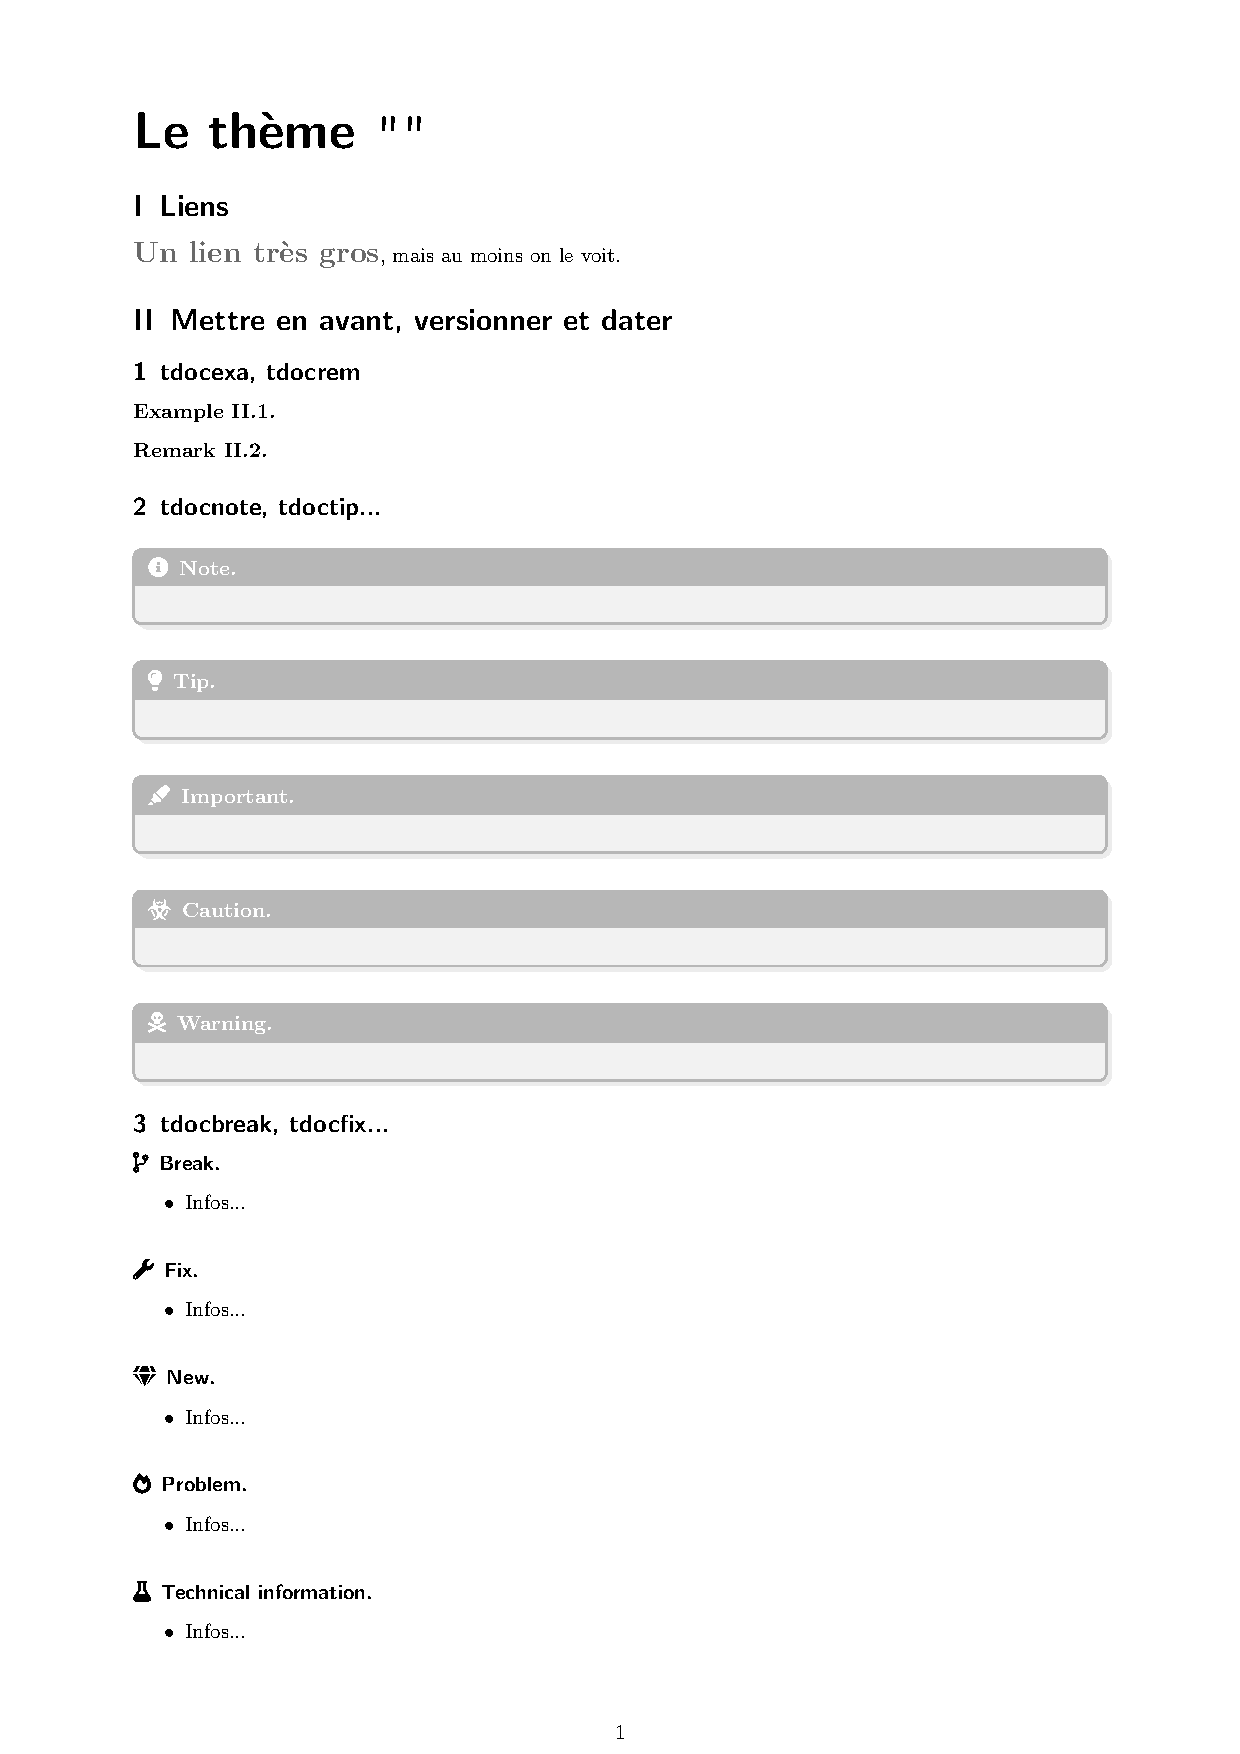
\includepdf{gallery-showcase-bw}

\includepdf{gallery-showcase-color}

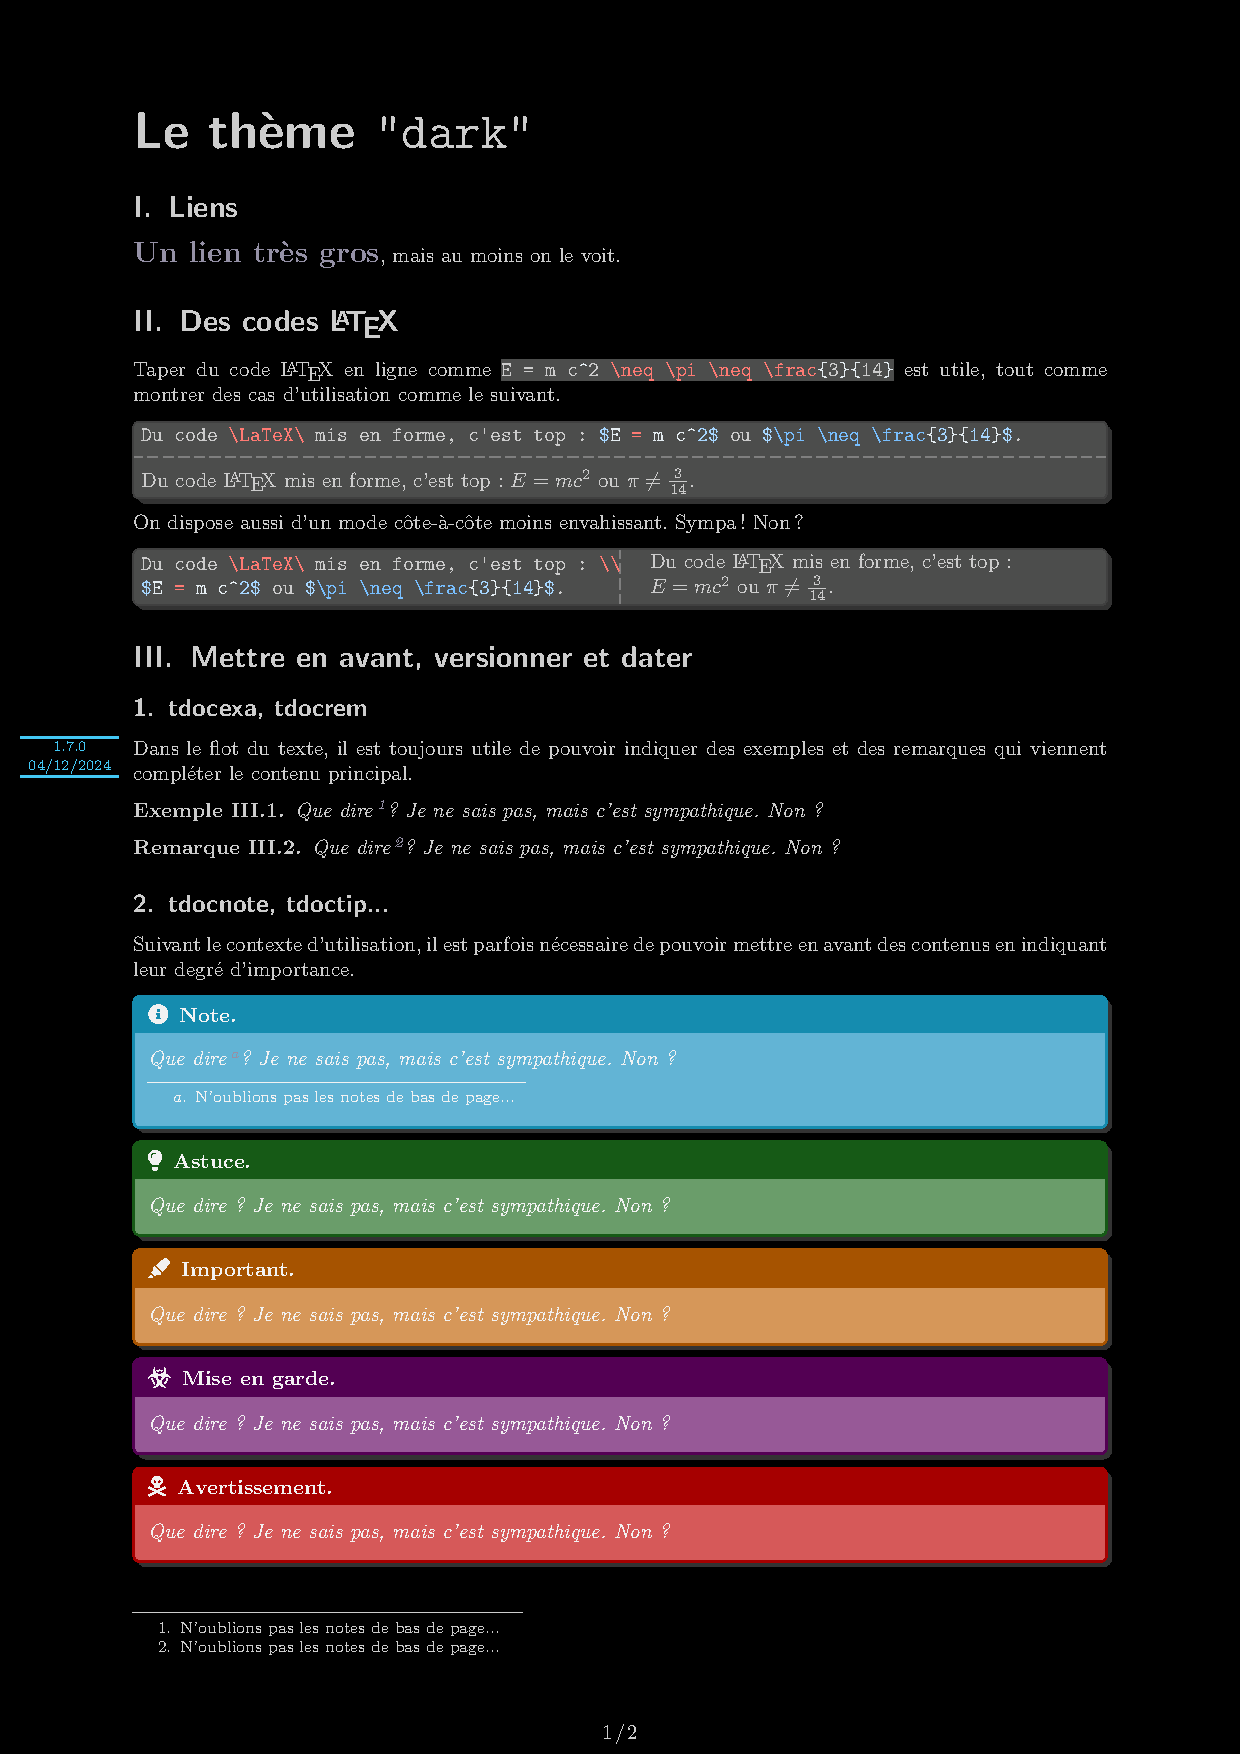
\includepdf{gallery-showcase-dark}

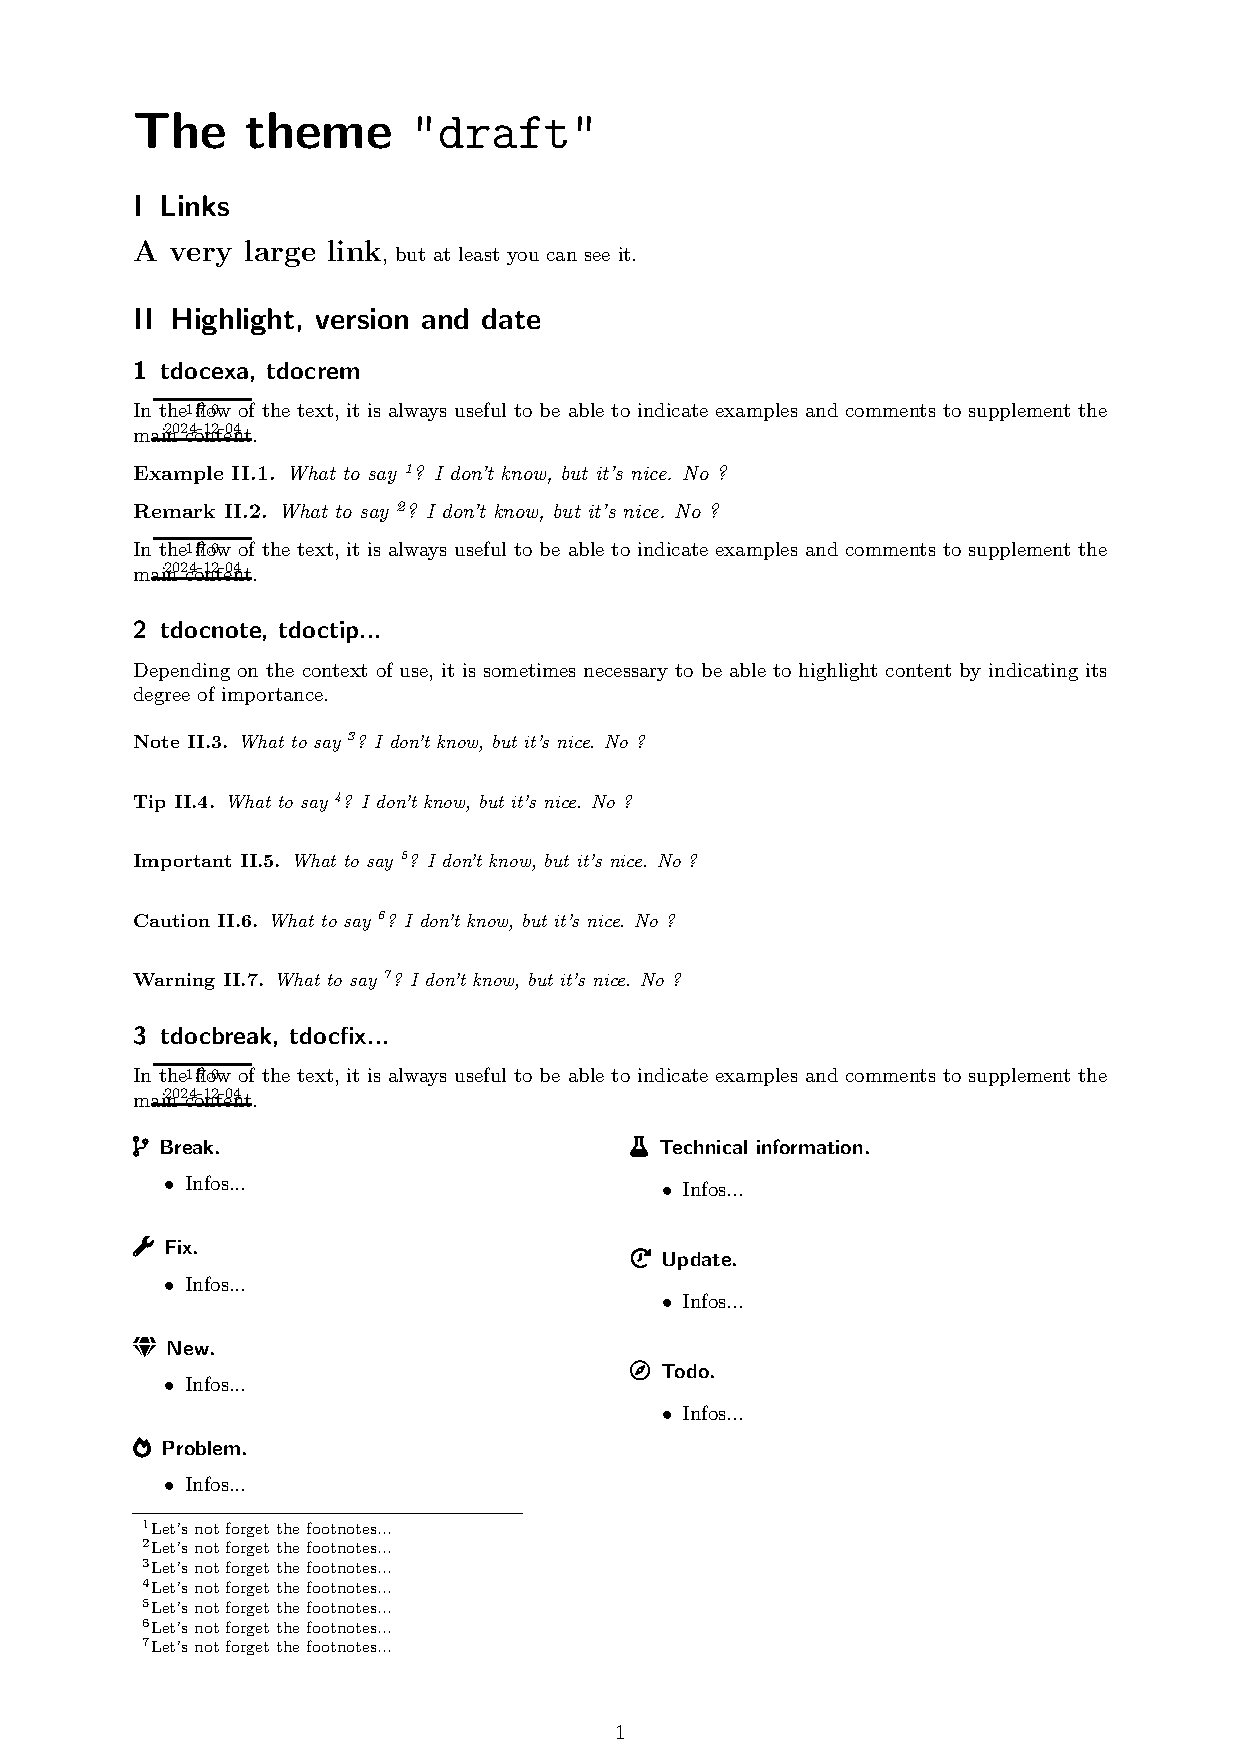
\includepdf{gallery-showcase-draft}

}

% --------------------------- %
% -- AT END DOCUMENT - END -- %
% --------------------------- %

\section{Highlighting content}

\begin{tdocnote}
    The environments presented in this section
    \footnote{
        The formatting comes from the \tdocpack{keytheorems} package.
    }
    add a short title indicating the type of information provided.
    This short text will always be translated into the language detected by the \thisproj\ class.
\end{tdocnote}


\subsection{Content in the reading flow}


% ------------------ %


\begin{tdocimp}
    All the environments presented in this section share the same counter, which will be reset to zero as soon as a section with a level at least equal to a \tdoclatexin|\section| is opened.
\end{tdocimp}


% ------------------ %


\subsubsection{Examples}

Numbered examples, if required, are indicated via \tdocenv{tdocexa}, which offers an optional argument for adding a mini-title.
Here are two possible uses.

\tdoclatexinput[\tdoctcb{sbs}]{examples-admonitions-exa.tex}



% ------------------ %


\begin{tdoctip}
    It can sometimes be useful to return to the line at the start of the content. The code below shows how to proceed (this trick also applies to the \verb#tdocrem# environment presented next). Note in passing that the numbering follows that of the previous example as desired.
\end{tdoctip}

\tdoclatexinput[\tdoctcb{sbs}]{examples-admonitions-exa-leavevmode.tex}



% \subsection{Content in the reading flow}

\subsubsection{Some remarks}

Everything happens via \tdocenv{tdocrem}, which works identically to the \tdocenv*{tdocexa} environment, as shown in the following example.

\tdoclatexinput[\tdoctcb{sbs}]{examples-admonitions-rmk.tex}



\subsection{Flashy content}
\label{tutodoc-admonitions}

\begin{tdocnote}
    The formatting proposed here is the default one, but others are possible by changing the theme: see the gallery of use cases in the appendix page \pageref{tutodoc-theme-gallery}.
    As for the icons, they are obtained via the \tdocpack{fontawesome5} package, and the \tdocmacro{tdocicon} macro manages the spacing in relation to the text.
    \footnote{
        For example,
        \tdoclatexin|\fbox{tdocicon{faBed}{Fatigued}}|
        produces
        \fbox{\tdocicon{\faBed}{Fatigued}}\,.
    }
\end{tdocnote}


\subsubsection{A tip}

The \tdocenv*{tdoctip} environment is used to give tips. Here's how to use it.

\tdoclatexinput[\tdoctcb{sbs},bottom=3pt,top=3pt]{examples-admonitions-tip.tex}



\smallskip


\begin{tdoctip}
    Sometimes, highlighted content can be reduced to a list. In this case, the formatting can be improved as follows where we use the \tdoclatexin{wide} option from the \tdocpack{enumitem} package.

    \tdoclatexinput[\tdoctcb{sbs},bottom=3pt,top=3pt]{examples-admonitions-leavevmode-items.tex}

\end{tdoctip}


\foreach \sectitle/\desc/\filename in {
    {Informative note}/%<-- Translate me!
    {The \tdocenv*{tdocnote} environment is used to highlight useful information. Here's how to use it.}/%<-- Translate me!
    note,
    %
    {Something important}/%<-- Translate me!
    {The \tdocenv*{tdocimp} environment is used to indicate something important but harmless.}/%<-- Translate me!
    important,
    %
    {Caution about a delicate point}/%<-- Translate me!
    {The \tdocenv*{tdoccaut} environment is used to indicate a delicate point to the user. Here's how to use it.}/% <-- Translate me!
    caution,
    %
    {Warning of danger}/%<-- Translate me!
    {The \tdocenv*{tdocwarn} environment is used to warn the user of a trap to avoid. Here's how to use it.}/%<-- Translate me!
    warn%
} {
    \subsubsection{\sectitle}

    \desc

    \tdoclatexinput[\tdoctcb{sbs},bottom=3pt,top=3pt]{examples-admonitions-\filename.tex}

}


\section{Specify packages, classes, macros or environments}

Here's what you can type semantically.


\begin{tdoclatex}[\tdoctcb{sbs}]
\tdoccls{myclass} is for...              \\
\tdocpack{mypackage} is for...           \\
\tdocmacro{onemacro} is for...           \\
\tdocenv{env} produces...                \\
\tdocenv[{[opt1]<opt2>}]{env}            \\
Just \tdocenv*{env}...                   \\
Finally \tdocenv*[{[opt1]<opt2>}]{env}...
        % For copy and paste.
\end{tdoclatex}


\begin{tdocrem}
    Unlike \tdocmacro{tdoclatexin}, \tdocmacro{tdocenv} and \tdocmacro{tdocenv*} macros don't color the text they produce.
    In addition, \tdoclatexin{\tdocenv{monenv}} produces \tdocenv{monenv} with spaces to allow line breaks if required.
\end{tdocrem}


\begin{tdocwarn}
    The optional argument of the \tdocmacro{tdocenv} macro is copied and pasted
    \footnote{
        Remember that almost anything is possible from now on.
    }
    when rendering. This may sometimes require the use of protective braces, as in the example above.
\end{tdocwarn}



\section{Origin of a prefix or suffix}

To explain the names chosen, there is nothing like indicating and explaining the short prefixes and suffixes used. This is easily done as follows.


\begin{tdoclatex}[\tdoctcb{sbs}]
\tdocpre{sup} relates to...      \\
\tdocprewhy{sup.erbe} means...   \\
\emph{\tdocprewhy{sup.er} for...}
\end{tdoclatex}


\begin{tdocrem}
    The choice of a full stop to split a word allows words with a hyphen to be used, as in \tdoclatexin+\tdocprewhy{bric.k-breaker}+ which gives \tdocprewhy{bric.k-breaker}.
\end{tdocrem}


\section{A real-life rendering}
\label{tutodoc-showcase}

It is sometimes useful to render code directly in the documentation. This type of rendering must be dissociable from the explanatory text.



\subsection{With a colored stripe}

\begin{tdocexa} [With default text]
    It can be useful to show a real rendering directly in a document.
    \footnote{
        Typically when making a demo.
    }
    This is done via \tdocenv{tdocshowcase} as follows.

    \tdoclatexinput[\tdoctcb{code}]{examples-showcase-default.tex}


    The result is the following rendering.
    \footnote{
        Behind the scenes, the strip is created effortlessly using the \tdocpack{clrstrip} package.
    }
\end{tdocexa}

\begin{tdocshowcase}
    \bfseries A bit of code \LaTeX.

    \bigskip

    \emph{\large End of the awful demo.}
\end{tdocshowcase}




\smallskip

\begin{tdocrem}
    See the section \ref{tutodoc-listing-latexshow} on page \pageref{tutodoc-listing-latexshow} to easily obtain code followed by its actual rendering as in the previous example.
\end{tdocrem}


\begin{tdocnote}
    The explanatory texts adapt to the language detected by \thisproj.
\end{tdocnote}


% ------------------ %


\begin{tdocexa}[Change the colors and/or the texts]
    \leavevmode

    \tdoclatexinput[\tdoctcb{code}]{examples-showcase-customized.tex}


    This will produce the following.

    \medskip

    \begin{tdocshowcase}[before = Mon début,
                     after  = Ma fin à moi,
                     color  = red]
    Bla, bla, bla, bla, bla, bla, bla, bla, bla, bla, bla, bla, bla...
\end{tdocshowcase}


\end{tdocexa}


\begin{tdocnote}
    In the previous example, the text uses the proposed darkened orange. On the other hand, red is used as a base to obtain the colors used for the strip: the transformations used depend on the theme chosen.%
    \footnote{
        For example, the themes \tdoclatexin{bw} and \tdoclatexin{draft} ignore the key \tdoclatexin{col-stripe}!
    }
    %
    You should also be aware that behind the scenes, the macro \tdocmacro{tdocruler} is used.

    \begin{tdoclatex}[\tdoctcb{std}]
        \tdocruler[red]{A decorated pseudo-title}
    \end{tdoclatex}
\end{tdocnote}


% ------------------ %


\begin{tdocwarn}
    With the default settings, if the code to be formatted begins with an opening bracket, use \tdocmacro{string} as in the following example.

    \tdoclatexinput[\tdoctcb{code}]{examples-showcase-hook.tex}


    This will produce the following.
\end{tdocwarn}


\begin{tdocshowcase}
    \string[Cela fonctionne...]
\end{tdocshowcase}




\subsection{Without a coloured strip}

The rendering of \tdocenv{tdocshowcase} with a coloured strip may not be suitable, or sometimes may not be acceptable despite the work done by \tdocpack{clrstrip}.
It is possible not to use a coloured strip, as we will see straight away.


\begin{tdocexa}
    The use of \tdocenv[{[nostripe]}]{tdocshowcase} indicate to not use \tdocpack{clrstrip}.
    Here is an example.

    \tdoclatexinput[\tdoctcb{code}]{examples-showcase-nostripe.tex}


    This will produce the following.

    \medskip

    \begin{tdocshowcase}[nostripe]
    Bla, bla, bla, bla, bla, bla, bla, bla, bla, bla, bla, bla, bla...
\end{tdocshowcase}


\end{tdocexa}


% ------------------ %


\begin{tdocexa}[Change the colors and/or the texts]
    \leavevmode

    \tdoclatexinput[\tdoctcb{code}]{examples-showcase-nostripe-customized.tex}


    This will produce the following horror.

    \medskip

    \begin{tdocshowcase}[nostripe,
                     before     = My beginning,
                     after      = My end,
                     col-stripe = green,
                     col-text   = purple]
    Bla, bla, bla, bla, bla, bla, bla, bla, bla, bla, bla, bla, bla...
\end{tdocshowcase}


\end{tdocexa}


\subsection{By importing the \LaTeX\ code}

To obtain renderings by importing the code from an external file, simply use the \tdocmacro{tdocshowcaseinput} macro whose option uses the syntax of that of \tdocenv{tdocshowcase} and the mandatory argument corresponds to the path of the file.


\begin{tdocexa}
    The following was obtained via \tdoclatexin+\tdocshowcaseinput{external.tex}+.

    \medskip

    \tdocshowcaseinput{examples-showcase-external.tex}


    \medskip

    As for \tdoclatexin+\tdocshowcaseinput[col-stripe = red, col-text = orange!75!black]{external.tex}+\,, this will produce the color change shown below.

    \medskip

    \tdocshowcaseinput[col-stripe = red, col-text = orange!75!black]{examples-showcase-external.tex}

\end{tdocexa}


\section{Use cases in \LaTeX}
\label{tutodoc-listing-latex}

Documenting a package or class is best done through use cases showing both the code and the corresponding result.
\footnote{
    Code is formatted using the \tdocpack{minted} and \tdocpack{tcolorbox} packages.
}


\subsection{\tdocquote{Inline} codes}
\label{tutodoc-listing-latex-inline}

The \tdocmacro{tdoclatexin} macro
\footnote{
    The name of the macro \tdocmacro{tdoclatexin} comes from \tdocquote{\tdocprewhy{in.line} \LaTeX}.
}
can be used to type inline code in a similar way to \tdocmacro{verb} or like a standard macro (see brace management in the last case below).
Here are some examples.


\begin{tdoclatex}[\tdoctcb{sbs}]
    1: \tdoclatexin|$a^b = c$|               \\
    2: \tdoclatexin+\tdoclatexin|$a^b = c$|+ \\
    3: \tdoclatexin{\tdoclatexin{$a^b = c$}}
\end{tdoclatex}


\begin{tdocnote}
    The \tdocmacro{tdoclatexin} macro can be used in a footnote: see below.
    \footnote{
        \tdoclatexin+$minted = TOP$+ has been typed \tdoclatexin|\tdoclatexin+$minted = TOP$+| in this footnote...
    }
    In addition, a background color is deliberately used to subtly highlight the codes \tdoclatexin#\LaTeX#\,.
\end{tdocnote}


% ------------------ %


\subsection{Directly typed codes}

\begin{tdocexa}[Side by side]
    Displaying a code and its rendering side by side is done as follows where the macro \tdocmacro{tdoctcb} allows you to just type \tdoclatexin{\tdoctcb{sbs}} instead of \tdoclatexin{listing side text} (\tdoclatexin#sbs# is for \tdocquote{\tdocprewhy{s.ide} \tdocprewhy{b.y} \tdocprewhy{s.ide}}\,, while \tdoclatexin#tcb# is the standard abbreviation for \texttt{tcolorbox}).

    \tdocbasicinputDOC*{examples-listing-latex-ABC.tex}

\end{tdocexa}


\begin{tdocnote}
	L'argument optionnel de l'environnement \tdocenv*{tdoclatex} doit être un style pour un \tdocmacro{tcblisting}. Par exemple, on peut faire les modifications suivantes si besoin.%
	\footnote{
		Cette documentation utilise ceci pour obtenir des rendus corrects de codes \LaTeX\ produisant des cadres ombrés : voir la section \ref{tutodoc-admonitions} page \pageref{tutodoc-admonitions}.
	}

	The optional argument of the \tdocenv*{tdoclatex} environment must be a style for a \tdocmacro{tcblisting}. For example, the following modifications can be made if required.
	\footnote{
		This documentation uses this to obtain correct renderings of \LaTeX\ codes producing shaded frames: see the section \ref{tutodoc-admonitions} on page \pageref{tutodoc-admonitions}.
	}

    \tdocbasicinputDOC*{examples-listing-latex-ABC-custom.tex}

\end{tdocnote}


% ------------------ %


\begin{tdocexa}[Following]
    \tdocenv{tdoclatex} produces the following result via the default option corresponding to \tdoclatexin#\tdoctcb{std}#\,.
    \footnote{
        \tdoclatexin{std} refers to the \tdocquote{standard} behaviour of \tdocpack{tcolorbox} in relation to the \tdocpack{minted} library.
    }

    \begin{tdoclatex}
        $A = B + C$
    \end{tdoclatex}
\end{tdocexa}


% ------------------ %


\begin{tdocexa}[Just the code]
    Via the option \tdoclatexin#\tdoctcb{code}#, we'll just get the code as shown below.

    \begin{tdoclatex}[\tdoctcb{code}]
        $A = B + C$
    \end{tdoclatex}
\end{tdocexa}


% ------------------ %


\begin{tdocwarn}
    With default formatting, if the code begins with an opening bracket, the default option must be explicitly indicated.
    \tdocbasicinputDOC{examples-listing-latex-strange.tex}


    \smallskip

    Another method is to use the \tdocmacro{string} primitive.
    \tdocbasicinputDOC{examples-listing-latex-strange-bis.tex}

\end{tdocwarn}


\subsection{Imported codes}

For the following codes, consider a file with the relative path \verb+examples-listing-xyz.tex+, and with the following contents.

\tdoclatexinput[\tdoctcb{code}]{examples-listing-latex-xyz.tex}


\medskip

The \tdocmacro{tdoclatexinput} macro, shown below, expects the path of a file and offers the same options as the \tdocenv*{tdoclatex} environment.


% ------------------ %


\begin{tdocexa}[Side by side]
    \leavevmode

    \begin{tdoclatex}[\tdoctcb{code}]
\tdoclatexinput[\tdoctcb{sbs}]{examples-listing-latex-xyz.tex}

    \end{tdoclatex}

    This produces the following layout.

    \tdoclatexinput[\tdoctcb{sbs}]{examples-listing-latex-xyz.tex}

\end{tdocexa}


% ------------------ %


\begin{tdocexa}[Following]
    \leavevmode

    \begin{tdoclatex}[\tdoctcb{code}]
\tdoclatexinput{examples-listing-latex-xyz.tex}

    \end{tdoclatex}

    This produces the following formatting where the default option is \tdoclatexin#\tdoctcb{std}#.

    \tdoclatexinput{examples-listing-latex-xyz.tex}

\end{tdocexa}


% ------------------ %


\begin{tdocexa}[Just the code]
    \leavevmode

    \begin{tdoclatex}[\tdoctcb{code}]
\tdoclatexinput[\tdoctcb{code}]{examples-listing-latex-xyz.tex}

    \end{tdoclatex}

    This produces the following layout.

    \tdoclatexinput[\tdoctcb{code}]{examples-listing-latex-xyz.tex}

\end{tdocexa}


% ------------------ %


\subsection{Imported codes put into practice}
\label{tutodoc-listing-latexshow}

\begin{tdocexa}[Showcase]
    The following comes from \tdoclatexin+\tdoclatexshow{examples-listing-xyz.tex}+.

    \medskip

    \begin{tdocshowcaseDOC}
        \tdoclatexshow{examples-listing-latex-xyz.tex}

    \end{tdocshowcaseDOC}
\end{tdocexa}


\begin{tdocnote}
    The default texts take into account the language detected by \thisproj.
\end{tdocnote}


% ------------------ %


\begin{tdocexa}[Changing the explanatory text]
    Using the key \tdoclatexin|explain|, you can use custom text. Thus, \tdoclatexin|tdoclatexshow[explain = Here is the rendering.]{examples-listing-xyz.tex}| will give the following.

    \medskip

    \begin{tdocshowcaseDOC}
        \tdoclatexshow[explain = Here is the rendering.]{examples-listing-latex-xyz.tex}

    \end{tdocshowcaseDOC}
\end{tdocexa}


% ------------------ %


\begin{tdocexa}[The options available]
    In addition to the explanatory text, it is also possible to use all the options of \tdocenv*{tdocshowcase} environment, see \ref{tutodoc-showcase} on page \pageref{tutodoc-showcase}.
    Here is an example to illustrate this.

    \medskip

    \tdoclatexinput[\tdoctcb{code}]{examples-listing-latex-latexshow-options.tex}


    \medskip

    This will produce the following.

    \medskip

    \begin{tdocshowcaseDOC}
        \tdoclatexshow[explain   = Ce qui vient est coloré...,
               before    = Rendu ci-après.,
               after     = Rendu fini.,
               col-stripe = orange,
               col-text   = blue!70!black]
               {examples-listing-latex-xyz.tex}


    \end{tdocshowcaseDOC}
\end{tdocexa}


\section{XXX}

\subsection{YYT}

ZZZ


\subsection{XXX}

YYY


\section{Indicate changes}
\label{tutodoc-changes}

To make it easier to monitor a project, it is essential to provide a history indicating the changes made when a new version is published.



\subsection{When?}
\label{tutodoc-changes-when}

You can either date something, or version it, in which case the version number can be dated.


% ------------------ %


\begin{tdocexa}[Dating new products]
    The \tdocmacro{tdocdate} macro is used to indicate a date in the margin, as in the following example.

    \tdoclatexshow{examples-version-n-change-dating.tex}

\end{tdocexa}


% ------------------ %


\begin{tdocexa}[Versioning new features, possibly with a date]
    Associating a version number with a new feature is done using the \tdocmacro{tdocversion} macro, with the colour and date being optional arguments.

    \tdoclatexshow{examples-version-n-change-versioning.tex}

\end{tdocexa}


\begin{tdocexa}[Caution with paragraph titles]
	The following example shows that a date and/or version must be placed just after a paragraph title, and not before it.

	\tdoclatexshow{examples-version-n-change-para-title.tex}

\end{tdocexa}


\begin{tdocexa}[Adjust vertical positioning]
	If required, you can modify the vertical offset used to place dates and versions in the margin, the default value being $(-8\,\mathit{pt})$.

	\tdoclatexshow{examples-version-n-change-manual-setting.tex}

\end{tdocexa}


\begin{tdocimp}
    \begin{enumerate}[wide]
        \item The \tdocmacro{tdocdate} and \tdocmacro{tdocversion} macros require two compilations.

        \item The final rendering of the dates takes into account the language detected by \thisproj{}: for example, if French is selected, the dates will be displayed in the format \texttt{DD/MM/YYYY}.
    \end{enumerate}
\end{tdocimp}


\begin{tdoccaut}
    Only the use of the digital format \tdoclatexin+YYYY-MM-DD+ is verified,
    \footnote{
        Technically, checking the validity of a date using \LaTeX3 presents no difficulty.
    }
    and this is a choice! Why? Quite simply because dating and versioning explanations should be done semi-automatically to avoid any human bugs.
\end{tdoccaut}


\subsection{What's new?}

\thisproj\ offers the macro \tdocmacro{tdocstartproj} and different environments to indicate quickly and clearly what has been done during the changes made, or to come.%
\footnote{
    The user doesn't need all the technical details.
}


\begin{tdocnote}
    For icons, see the note at the beginning of the section \ref{tutodoc-admonitions} on page \pageref{tutodoc-admonitions}.
\end{tdocnote}


\subsubsection{Sobriety first}

\foreach \exatitle/\filename in {
    {Just for the very first version}/%<-- Translate me!
        first,
    {For new features}/% <-- Translate me!
        new,
    {For updates}/% <-- Translate me!
        update,
    {For breaks}/% <-- Translate me!
        break,
    {For problems}/% <-- Translate me!
        pb,
    {For fixes}/% <-- Translate me!
        fix,
    {Roadmap}/% <-- Translate me!
        todo,
    {Technical information}/% <-- Translate me!
        tech,
    {Selectable themes with an icon}/% <-- Translate me!
        user-choice-icon,
    {Selectable themes without icons}/%<-- Translate me!
        user-choice%
} {
    \begin{tdocexa}[\exatitle]
        \leavevmode

        \tdoclatexinput[\tdoctcb{sbs}]{examples-version-n-change-chges-\filename.tex}

    \end{tdocexa}
}


\subsubsection{De la couleur si besoin}

\subsubsection{Color if necessary}

It may be useful to highlight certain changes: this can only be done by modifying the content color.

\foreach \exatitle/\filename in {
    {A flashy first version}/%<-- Translate me!
        first,
    {Outstanding fixes}/% <-- Translate me!
        fix%
} {
    \begin{tdocexa}[\exatitle]
        \leavevmode

        \tdoclatexinput[\tdoctcb{sbs}]{examples-version-n-change-color-chges-\filename.tex}

    \end{tdocexa}
}


\subsection{The what and the when}

The optional keys \tdoclatexin{col}\,, \tdoclatexin{date} and \tdoclatexin{version} allow to date and version a change of a particular type.
Here are some examples of use.

\tdoclatexshow{examples-version-n-change-what-n-when.tex}



\section{Ornament}

Let's finish this documentation with a small formatting tool that is very useful.


\begin{tdoclatex}[\tdoctcb{sbs}]
Bla, bla, bla...

\tdocsep % Practical for demarcation.

This works with enumerations.

\begin{itemize}
    \item Underline.
\end{itemize}

\tdocsep % Uniform behaviour.

Ble, ble, ble...
\end{tdoclatex}


\section{Contribute}

\begin{tdocnote}
    \textbf{You don't need to be a coder to take part in translations}, including those that are useful for the running of \thisproj.
\end{tdocnote}


%\section{Contribute}

\subsection{Complete the translations}

\begin{tdocnote}
    The author of \thisproj\ manages the French and English versions of the translations.
\end{tdocnote}


\begin{tdoccaut}
    Although we're going to explain how to translate the documentation, it doesn't seem relevant to do so, as English should suffice these days.%
    \footnote{
      The existence of a French version is simply a consequence of the native language of the author of \thisproj.
    }
\end{tdoccaut}


\begin{figure}[ht]
    \centering
    \contribtranslatedirtree\
    \caption{Simplified view of the translation folder}
    \label{tutodoc-contrib-translate-dir}
\end{figure}


The translations are roughly organized as in figure \ref{tutodoc-contrib-translate-dir} where only the folders important for the translations have been \tdocquote{opened}\,.%}.
\footnote{
    This was the organization on October 5, 2024, but it's still relevant today.
}
\textbf{A little further down, the section \ref{tutodoc-contrib-translate} explains how to add new translations}.


\subsubsection{The \texttt{fr} and \texttt{en} folders}

These two folders, managed by the author of \thisproj, have the same organization; they contain files that are easy to translate even if you're not a coder.


\subsubsection{The \texttt{changes} folder}

This folder is a communication tool where important changes are indicated without dwelling on minor modifications specific to one or more translations.


\subsubsection{The \texttt{status} folder}

This folder is used to keep track of translations from the project's point of view. Everything is done via well-commented \verb#YAML# files, readable by a non-coder.


\subsubsection{The \texttt{README.md} and \texttt{LICENSE.txt} files}

The \texttt{LICENSE.txt} file is aptly named, while the \texttt{README.md} file takes up in English the important points of what is said in this section about new translations.


\subsubsection{New translations}
\label{tutodoc-contrib-translate}

\begin{tdocimp}
    The \verb#api# folder contains translations relating to the functionalities of \thisproj.
    Here you'll find \verb#TXT# files for editing with a text or code editor, but not with a word processor.
    The content of these files uses commented lines in English to explain what \thisproj\ will do; these lines begin with \verb#//#\,. Here's an extract from such a file, where translations are made after each \,$=$\ sign, without touching the preceding, as this initial piece is used internally by the \thisproj code.

    \tdocsep
    \vspace{-10pt}
    \begin{verbatim}
    // #1: year  in format YYYY like 2023.
    // #2: month in format MM   like 04.
    // #3: day   in format DD   like 29.
    date = #1-#2-#3

    // #1: the idea is to produce one text like
    //     "this word means #1 in English".
    in_EN = #1 in english\end{verbatim}
\end{tdocimp}


\begin{tdocnote}
    The \verb#doc# folder is reserved for documentation. It contains files of type \verb#TEX# that can be compiled directly for real-time validation of translations.
\end{tdocnote}


\begin{tdocwarn}
    Only start from one of the \verb#fr# and \verb#en# folders, as these are the responsibility of the \thisproj\ author.
\end{tdocwarn}


\medskip


\emph{\textbf{Let's say you want to add support for Italian from files written in English.}}%
\footnote{
    As mentioned above, there is no real need for the \texttt{doc} documentation folder.
}


\paragraph{Method 1 : \git.}

\begin{enumerate}
      \item Obtain the entire project folder via \thisrepo\,.
    Do not use the \verb#main# branch, which is used to freeze the latest stable versions of projects in the single \thismonorepo\ repository,.

      \item In the \verb#tutodoc/contrib/translate# folder, create a \verb#it# copy of the \verb#en# folder, with the short name of the language documented in
      \href{https://en.wikipedia.org/wiki/IETF_language_tag#List_of_common_primary_language_subtags}%
           {the page \tdocquote{IIETF language tag}}
      from \texttt{Wikipedia}.

      \item Once the translation is complete in the \verb#it# folder, you'll need to communicate it via \thisrepo\ using a classic \verb#git push#\,.
\end{enumerate}


\paragraph{Method 2 : communicate by e-mail.}

\begin{enumerate}
      \item By e-mail with the \mailsubject{en FOR italian}, request a version of the English translations (note the use of the English name for the new language).
    Be sure to respect the subject of the e-mail, as the author of \thisproj\ automates the pre-processing of this type of e-mail.

      \item You will receive a folder named \verb#italian# containing the English version of the latest translations.
    This folder will be the place for your contribution.

      \item Once the translation is complete, you will need to compress your \verb#italian# file in \verb#zip# or \verb#rar# format before sending it by e-mail with the \mailsubject{italian}\,.
\end{enumerate}


%\section{Contribute}

\subsection{Improving the source code}

\begin{tdocimp}
    If you want to participate in \thisproj\, you'll need to use the \LaTeX3 programming paradigm.
\end{tdocimp}


Participation as a coder is made via the \thisrepo\ repository corresponding to the \verb#tutodoc# development branch.


\begin{tdoccaut}
Do not use the \verb#main# branch, which is used to freeze the latest stable versions of projects in the single \thismonorepo\ repository.
\end{tdoccaut}


\section{History}

\small

\begin{tdocbreak}[version = 1.7.0, date = 2024-12-04]
	\item Format: the \tdoccls{scrartcl} class replaces the venerable \tdoccls{article}. This implies better placement of the margin notes with the options retained for loading \tdoccls{scrartcl}.

	\item \LaTeX\ code: the macro \tdocmacro{tdocinlatex} has been renamed \tdocmacro{tdoclatexin}.

	\item Color key names will be hyphenated where necessary: this implies the following changes.
	%
	\begin{enumerate}
		\item Indicate the latest changes: the \tdoclatexin{colchges} option of the environments has been renamed \tdoclatexin{col-chges}.

		\item Showcases: for the environment \tdocenv*{tdocshowcase} and the macro \tdocmacro{tdocshowcaseinput}, the \tdoclatexin{colstripe} and  \tdoclatexin{coltext} options have been renamed \tdoclatexin{col-stripe} and \tdoclatexin{col-text}\,.
	\end{enumerate}
\end{tdocbreak}


\begin{tdocfix}
	\item Admonitions: for the \tdocmacro{newkeytheorem} used with the \tdoclatexin{draft} theme, \tdoclatexin{postheadhook = \leavevmode} has been added (this is necessary because the content can naturally be of the list type).
\end{tdocfix}


\begin{tdocnew}
	\item Documentation: addition of a section listing dependencies.

	\item Class options.
	%
	\begin{enumerate}
		\item Options not specific to \thisproj\ are passed on to the class in charge of general formatting.

		\item The \tdoccls{scrartcl} options \tdoclatexin{fontsize} and \tdoclatexin{DIV} can't be used because their values are fixed by \thisproj.
	\end{enumerate}

	\item The macro \tdocmacro{tdocinEN} respects the English linguistic rules.

	\item Indicate the latest changes.
	%
	\begin{enumerate}
		\item Add the environment \tdocenv{tdoctodo}\,.

		\item Each environment has a new option \tdoclatexin{col} for the colour of the content indicating changes.
	\end{enumerate}
\end{tdocnew}


\begin{tdocupdate}
	\item \tdoclatexin{draft} theme and changes: the environments for the latest changes stop to use icons.

	\item Documentation: the theme gallery uses a better fake example.
\end{tdocupdate}



\begin{tdoctech}
	\item Simplified organisation of configuration files in the final project.
	%
	\begin{enumerate}
		\item \texttt{CSS}-like: use of one file per theme with a name like \texttt{tutodoc-bw.css.cls}\,.

		\item Locale: use of names like \texttt{tutodoc-en.loc.cls}\,.
	\end{enumerate}
\end{tdoctech}

\tdocsep


% ------------------ %


\begin{tdocnew}[version = 1.6.2, date = 2024-10-30]
	\item The macros \tdocmacro{tdocdate} and \tdocmacro{tdocversion} has a new final optional argument \tdoclatexin{<voffset>} to choose a specific vertical offset.

	\item Better environments to indicate the changes made.
	\begin{enumerate}
        \item The new optional keys \tdoclatexin{col}\,, \tdoclatexin{date} and \tdoclatexin{version} allow to date and version a change of a specific topic.

        \item Use of \tdocmacro{paragraph} for the title.
	\end{enumerate}
\end{tdocnew}


\begin{tdocupdate}
	\item Version and changes: the font of the margin notes will always have a normal shape.

	\item Ornament: use of a \tdoclatexin{\cleaders} to avoid orphean rules at the bottom of a page.
\end{tdocupdate}

\tdocsep


% ------------------ %


\begin{tdoctech}[version = 1.6.1, date = 2024-10-28]
    \item The naming rules of \ctan\ need the use of \trademark{CSS} files named \verb+tutodoc-*.css.cls.sty+\,.
\end{tdoctech}

\tdocsep


% ------------------ %


\begin{tdocbreak}[version = 1.6.0, date = 2024-10-27]
    \item The \tdocenv*{showcase} environment and its descendants: the \tdoclatexin{color} key has been renamed \tdoclatexin{col-stripe}.

    \item The macro \tdocmacro{tdoclinkcolor} has been renamed \tdoclatexin{tutodoc@link@color} for internal use.
\end{tdocbreak}


\begin{tdocnew}
    \item The \tdoclatexin{theme} class option allows you to choose different formatting themes.

    \item Change log: addition of the \tdocenv*{tdoctech} environment for technical information.

    \item The \tdocenv*{showcase} environment and its descendants: the \tdoclatexin{col-text} key can also be used to change the text color.

    \item The new functionalities have been documented.
\end{tdocnew}


\begin{tdocupdate}
    \item Change log: the \tdocenv*{tdocupdate} environment uses the icon
    \raisebox{0pt}[0pt][0pt]{\fbox{\reflectbox{\faHistory}}}
    instead of
    \raisebox{0pt}[0pt][0pt]{\fbox{\faMagic}}\,.
\end{tdocupdate}


\begin{tdocfix}
    \item The Spanish translations were not included in the previous version! Don't laugh too hard...
\end{tdocfix}

\tdocsep


% ------------------ %


\begin{tdoctech}[version = 1.5.0, date = 2024-10-19]
    \item Version 3 of \tdocpack{minted} is taken into account.
\end{tdoctech}


\begin{tdocbreak}
    \item The \thisproj\ class replaces the now-defunct \thisproj\ package (for the moment, the young class offers no specific options).

    \item The \tdocmacro{tdocruler} macro is now used via \tdoclatexin{\tdocruler[<color>]{<text>}} (remember that the old syntax was \tdoclatexin{\tdocruler{<text>}{<color>}}).
\end{tdocbreak}


\begin{tdocnew}
    \item The class is usable in Spanish.

    \item The documentation contains a new section explaining how to contribute.
\end{tdocnew}


\begin{tdocfix}
    \item The \tdocmacro{tdocdate} macro did not handle date format and formatting.

    \item Colored frames did not color text after a page break.
\end{tdocfix}

\tdocsep


% ------------------ %


\begin{tdocbreak}[version = 1.4.0, date = 2024-09-28]
    \item The \tdocenv*{tdoccaution} environment has been renamed \tdocenv*{tdoccaut} for simplified input.

    \item Content highlighting: examples and remarks, indicated via the \tdocenv*{tdocexa} and \tdocenv*{tdocrem} environments, are always numbered using a common counter.

    \item The unused macro \tdocmacro{tdocxspace} has been deleted.
\end{tdocbreak}


\begin{tdocnew}
    \item Change log: the \tdocmacro{tdocstartproj} macro is used to manage the case of the first public version.

    \item Code factorization: the \tdocmacro{tdocicon} macro is responsible for adding icons in front of text.
\end{tdocnew}


\begin{tdocupdate}
    \item Colors: the \tdocmacro{tdocdarkcolor} and \tdocmacro{tdoclightcolor} macros offer an optional argument.
    \begin{enumerate}
        \item \tdocmacro{tdocdarkcolor}: the amount of color in relation to black can be optionally defined.

        \item \tdocmacro{tdoclightcolor}: the transparency rate can be optionally defined.
    \end{enumerate}

    \item Content highlighting: reduced space around content in colored frames.

    \item Versioning: better vertical spacing thanks to \tdocmacro{vphantom}.
\end{tdocupdate}

\tdocsep


% ------------------ %


\begin{tdocnew}[version = 1.3.1, date = 2024-09-26]
    \item Star version of \tdocmacro{tdocenv} to display only the environment name.
\end{tdocnew}

\tdocsep


% ------------------ %


\begin{tdoctech}[version = 1.3.0, date = 2024-09-25]
    \item Version 3 of \tdocpack{minted} cannot be used for the moment as it contains bugs: see \url{https://github.com/gpoore/minted/issues/401}. We therefore force temporarily the use of version 2 of \tdocpack{minted}.
\end{tdoctech}


\begin{tdocbreak}
    \item The \tdocenv*{tdocimportant} environment has been renamed \tdocenv*{tdocimp} for simplified input.
\end{tdocbreak}


\begin{tdocnew}
    \item Change log: proposed environments use icons.


    \item Content highlighting: colored frames with icons are proposed for the following environments.
    %
    \begin{tasks}[label=\arabic*.](3)
        \task \tdocenv*{tdoccaution}
        \task \tdocenv*{tdocimp}
        \task \tdocenv*{tdocnote}
        \task \tdocenv*{tdoctip}
        \task \tdocenv*{tdocwarn}
    \end{tasks}
\end{tdocnew}

\tdocsep


% ------------------ %


\begin{tdocupdate}[version = 1.2.0-a, date = 2024-08-23]
    \item \tdocmacro{tdocversion}
    \begin{enumerate}
        \item The version number is above the date.

        \item The spacing is better managed when the date is absent.
    \end{enumerate}
\end{tdocupdate}


\begin{tdocfix}
    \item Content highlighting: the French translations of \tdocinEN*{caution} and \tdocinEN*{danger} were incorrect.
\end{tdocfix}

\tdocsep


% ------------------ %


\begin{tdocnew}[version = 1.1.0, date = 2024-01-06]
    \item Change log: two new environments.
    \begin{enumerate}
        \item \tdocenv{tdocbreak} for breaking changes which are not backward compatible.

        \item \tdocenv{tdocprob} for identified problems.
    \end{enumerate}

    \item \tdocmacro{tdoclatexin}: a light yellow is used as the background color.
\end{tdocnew}

\tdocsep


% ------------------ %


\begin{tdocfix}[version = 1.0.1, date = 2023-12-08]
    \item \tdocmacro{tdocenv}: spacing is now correct, even if the \tdocpack{babel} package is not loaded with the French language.

    \item \tdocenv[{[nostripe]}]{tdocshowcase} : page breaks around \tdocquote{framing} lines should be rare from now on.
\end{tdocfix}

\tdocsep


% ------------------ %


\tdocversion{1.0.0}[2023-11-29]
\tdocstartproj{First public version of the project.}

\end{document}
